\documentclass[article, 11pt]{IEEEtran}   %Document is an article, 11 pt font, and follows IEEE format

%Packages
\usepackage{hyperref}         %hyperlinks
\usepackage{graphicx}         %images
\usepackage{float}            %figure placement
\usepackage[caption=false,font=footnotesize]{subfig}  %labeled sub-figures
\usepackage{gensymb}          %symbols
\usepackage{amsmath,amssymb}  %math
\usepackage{booktabs}         %tables
\usepackage{tikz}             %diagrams
\usetikzlibrary{arrows.meta,positioning}
\usepackage[utf8]{inputenc}
\usepackage[T1]{fontenc}
\usepackage[english]{babel}
\hypersetup{hidelinks}
\graphicspath{{imgs/}}

\begin{document}

\title{Modeling and Simulation of a Rocket in the Pitch Plane:\\ Stability, Coupling and Gain Selection}

\author{\IEEEauthorblockN{Jos\'e Barreno\\Luis Guzm\'an\\Byron Garc\'ia\\Jos\'e Rivera}
\IEEEauthorblockA{\\Universidad Galileo, Systems Theory II\\Guatemala, Guatemala}}

\maketitle

%====================================================================
\begin{abstract}
A rocket must not only accelerate, it must also point in the right direction, this work studies the linear model of a rocket in the pitch plane, with two inputs (an axial acceleration command and a pitch angle command), two measured outputs (an accelerometer and an inertial unit) and two control gains whose effect is analyzed, the transfer matrix is obtained, and stability, the time and frequency response, the coupling between channels, observability and controllability are studied, from which a range of gains and a sampling period are chosen, the rocket turns out to be unstable by nature, since the aerodynamics tend to overturn it, and the nozzle is what stabilizes it, with the starting gains gravity couples the two channels strongly, so that tilting the rocket takes away more acceleration than the thrust provides, the recommended range of gains reduces the overshoot and the settling time considerably and spreads the coupling more evenly between the two channels, at the cost of using almost all of the nozzle travel, a sampling period for the on-board computer is found to be sufficient, with a comfortable margin even when the computation delay is included, it is also discussed how the model would change with variable mass and with a yaw channel, since they are models closer to reality.
\end{abstract}

%====================================================================
\section{Introduction}
For a space mission to succeed it is not enough for the rocket to accelerate correctly, it must also point correctly, an error of a few degrees in attitude during the ascent becomes deviations of kilometers when the payload is inserted into orbit, and in aerodynamic loads that can destroy the structure, that is why a rocket is not a single-input single-output system, it is a \emph{multivariable} (MIMO) system~\cite{skogestad}, with a thrust channel that governs the acceleration and a steering channel that governs the pitch angle.

The two channels are not independent, the nozzle that corrects the direction also deflects the thrust and, when the rocket tilts, gravity takes away axial acceleration, and an increase in thrust, in the presence of a small engine misalignment, disturbs the attitude, this cross interaction (coupling) is the central phenomenon of this work, one way to control the direction is to orient the nozzle, there are others such as fins, vernier rockets and jet vanes~\cite{nasa}, here the gimbaled thrust is modeled with the classical hypotheses of a linearized pitch model~\cite{wie,greensite}.

This work follows the rocket from its model to the choice of its controller, it first describes what each part of the model does and how the two channels are connected, then it asks whether the rocket is stable and for which values of the gains, how strongly and at which frequencies the channels are coupled, and when it is reasonable to treat them as independent, after that it checks whether the whole state can be \emph{seen} and \emph{moved} with the available sensors and actuators, with that information it selects the gains and the sampling period, and finally it considers what would change if the mass decreased during flight or if yaw were included.


The working hypothesis is that gravity dominates the coupling, that $K_2$ (nozzle) governs stability and attitude while $K_1$ (engine) governs acceleration, and that there is a range of $(K_1,K_2)$ with a stable, fast response and acceptable nozzle use and coupling, the methodology combines the state-space model, the transfer matrix, time simulation, frequency analysis and a sampled model, a well-defined gain region and a sampling period with enough margin are expected.

%====================================================================
\section{Methodology}

\subsection{Model}
Only the pitch plane is modeled during the atmospheric phase of the ascent, with the usual hypotheses of a linearized model, motion in the plane, small angles ($\sin\theta\approx\theta$), mass, inertia and dynamic pressure constant in the analysis window, the engine responds with a first-order lag of time constant $\tau_m$ (an exponential rise, without dead time) and the nozzle servo with $\tau_s\ll\tau_m$, and a rigid fuselage without propellant sloshing, the state is $x=[a,\theta,\omega,\delta]^T$, axial acceleration, pitch angle, pitch rate and nozzle deflection, the inputs are $u_1$ (axial acceleration command, in \%) and $u_2$ (angle command, in rad), the measured outputs are $y=[a,\theta]^T$, with the gains already incorporated in the model,
\begin{align}
\dot a &= -\tfrac{1+K_1k_a}{\tau_m}\,a-c_\theta\,\theta+\tfrac{K_1k_a}{\tau_m}\,u_1,\label{eq:a}\\
\dot\theta &= \omega,\label{eq:th}\\
\dot\omega &= \mu\,\theta-a_d\,\omega+k_\delta\,\delta+k_\varepsilon\,a,\label{eq:om}\\
\dot\delta &= -\tfrac{1}{\tau_s}\,\delta-\tfrac{K_2}{\tau_s}\,\theta-\tfrac{\lambda K_2}{\tau_s}\,\omega+\tfrac{K_2}{\tau_s}\,u_2.\label{eq:de}
\end{align}
Behind the model there is a controller, with the laws
\begin{align}
v_1&=K_1(u_1-a),\label{eq:v1}\\
v_2&=K_2(u_2-\theta-\lambda\omega),\label{eq:v2}
\end{align}
where $\lambda\omega$ adds damping, so $K_1$ and $K_2$ appear \emph{inside} the matrices of the model, changing a gain changes the dynamics of the rocket in closed loop, the nominal values are summarized in Table~\ref{tab:param}, the starting gains are $K_1=1$, $K_2=0.5$ and the sampling period is $T=0.05$ s.

\begin{table}[!t]
\centering\small
\caption{Nominal parameters of the model.}\label{tab:param}
\begin{tabular}{p{0.9cm}p{2.4cm}p{3.6cm}}
\toprule
Symbol & Value & Physical role\\
\midrule
$k_a$ & 0.0655 (m/s$^2$)/\% & thrust actuator gain\\
$1/\tau_m$ & 1.0672 s$^{-1}$ & engine speed ($\tau_m\approx0.94$ s)\\
$c_\theta$ & 9.81 (m/s$^2$)/rad & gravity, loss of acceleration when tilted\\
$\mu$ & 1.20 s$^{-2}$ & aerodynamic stiffness (destabilizing)\\
$a_d$ & 0.35 s$^{-1}$ & aerodynamic damping\\
$k_\delta$ & 8.50 s$^{-2}$/rad & nozzle effectiveness\\
$k_\varepsilon$ & 0.12 rad/m & thrust misalignment\\
$1/\tau_s$ & 20 s$^{-1}$ & servo speed ($\tau_s=0.05$ s)\\
$\lambda$ & 0.60 s & weight of $\omega$ in the IMU\\
\bottomrule
\end{tabular}
\end{table}

\subsection{Tools and procedure}
All the computation was done in Python (NumPy, SciPy, SymPy and Matplotlib), with one function for each type of analysis, the transfer matrix
\begin{equation}
G(p)=C(pI-A)^{-1}B,
\end{equation}
where $p$ is the Laplace variable, is obtained symbolically and numerically, stability is studied with the Routh--Hurwitz criterion~\cite{ogata} and verified against the direct computation of the eigenvalues at 4941 pairs $(K_1,K_2)$, with no disagreement, the time responses are simulated with SciPy, the frequency response is obtained by evaluating $G(j\omega)$ between $10^{-3}$ and $10^{3}$ rad/s.

When effects with different units have to be compared (acceleration in m/s$^2$ and angle in rad) steps of $u_1=10\%$ thrust and $u_2=5^\circ$ are applied, these magnitudes are a choice of the team, they were chosen to keep the pitch angle and the nozzle deflection within a few degrees, where the linear model is valid, the two coupling percentages depend on the ratio $u_2/u_1$, so they are reported for this pair of steps.

Sampling is modeled by separating the rocket (plant, continuous) from the controller (the computer), only the feedback is sampled, every $T$ seconds (the sampling period, 0.05 s as the starting value) the computer reads the sensors and computes a command, and holds it constant until the next sample (zero-order hold, like a real D/A converter), if the already closed matrix $A$ were discretized, the controller and the rocket would be mixed and the result would be misleading, two cases are studied, an instantaneous computer and a one-sample delay, discrete stability is judged with the spectral radius (largest modulus of the eigenvalues), less than 1 is stable~\cite{franklin}.

%====================================================================
\section{Results and Discussion}

\subsection{Structure and dynamics of the rocket}
\subsubsection{The blocks}
The system has five parts, and the signal goes through them in this order, the \emph{sensors}, an accelerometer and an IMU, measure $a$ and $\theta$ (and $\omega$, which the IMU also delivers) as continuous analog signals, an \emph{A/D} (analog-to-digital) converter, at the input of the computer, takes a reading of those signals every $T$ seconds and converts it into numbers, the \emph{on-board computer} works only with those numbers, it receives the commands $u_1$ and $u_2$ (trajectory tracking data), compares them with what is measured and applies the gains $K_1$ and $K_2$ to compute the commands $v_1$ and $v_2$, a \emph{D/A} (digital-to-analog) converter, at the output of the computer, transforms those commands into analog signals and holds each one constant until the next sample, the \emph{power amplifiers} raise those signals to the level needed by the engine and the nozzle servo, finally there is the \emph{rocket dynamics}, continuous, whose outputs return to the sensors, sampling therefore occurs at the two interfaces of the computer, the input A/D and the output D/A, between them everything is discrete, and the rest of the loop (amplifiers, engine, servo, rocket and sensors) is continuous, the model assumes ideal conversions, it ignores quantization and conversion time, and keeps only the effect of the period $T$ and of holding the command.

\subsubsection{The cause--effect chain}
Equations~(\ref{eq:a})--(\ref{eq:de}) read like sentences (Fig.~\ref{fig:cadena}), moving the nozzle ($\delta$) produces a moment that makes the rocket rotate ($\omega$) and, by integrating, tilt ($\theta$), this is the main attitude path,
\begin{equation}
u_2\to\delta\to\omega\to\theta,
\end{equation}
the tilt has two consequences, the first is the \emph{gravity coupling}, part of the weight becomes aligned with the axis and takes away acceleration ($-c_\theta\theta$ in Eq.~\ref{eq:a}), so \emph{tilting the rocket reduces its axial acceleration}, the second is the aerodynamic overturning $\mu\theta$ in Eq.~(\ref{eq:om}), with $\mu=1.2>0$, the more tilted, the more the air pushes it to tilt even more, like an arrow with the feathers on backwards, which is why the rocket is \emph{unstable by nature}, in the opposite direction, thrust ($u_1\to a$) feeds $\dot\omega$ through $k_\varepsilon$, accelerating tilts the rocket a little (coupling $u_1\to\theta$), the rest of the analysis examines this chain from different angles.

\begin{figure}[!t]
\centering
\resizebox{\columnwidth}{!}{%
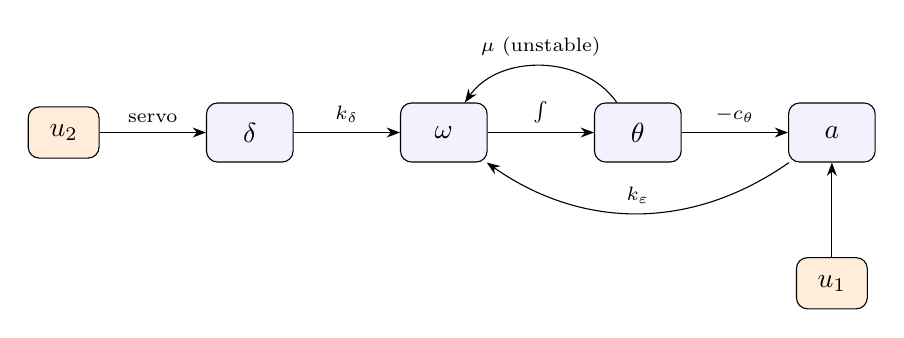
\begin{tikzpicture}[>=Stealth,node distance=1.35cm,
  box/.style={draw,rounded corners,minimum width=1.1cm,minimum height=0.75cm,fill=blue!5},
  inp/.style={draw,rounded corners,minimum width=0.9cm,minimum height=0.65cm,fill=orange!15}]
  \node[inp] (u2) {$u_2$};
  \node[box,right=of u2] (d) {$\delta$};
  \node[box,right=of d] (w) {$\omega$};
  \node[box,right=of w] (t) {$\theta$};
  \node[box,right=of t] (a) {$a$};
  \node[inp,below=1.2cm of a] (u1) {$u_1$};
  \draw[->] (u2)--(d) node[midway,above,font=\scriptsize]{servo};
  \draw[->] (d)--(w) node[midway,above,font=\scriptsize]{$k_\delta$};
  \draw[->] (w)--(t) node[midway,above,font=\scriptsize]{$\int$};
  \draw[->] (t)--(a) node[midway,above,font=\scriptsize]{$-c_\theta$};
  \draw[->] (u1)--(a);
  \draw[->] (a) to[bend left=35] node[midway,above,font=\scriptsize]{$k_\varepsilon$} (w);
  \draw[->] (t) to[bend right=55] node[midway,above,font=\scriptsize]{$\mu$ (unstable)} (w);
\end{tikzpicture}}
\caption{Cause--effect chain of the rocket, the arrows $-c_\theta$ and $k_\varepsilon$ are the two couplings between channels.}\label{fig:cadena}
\end{figure}

\subsubsection{The role of $K_1$ and $K_2$}
$K_1$ belongs to the engine channel, it appears in the coefficient $(1+K_1k_a)/\tau_m$ of Eq.~(\ref{eq:a}), when $K_1$ goes from 1 to 20, that coefficient goes from 1.14 to 2.46 s$^{-1}$, the characteristic time of the engine drops from 0.88 s to 0.41 s and the final acceleration per unit of command rises from 0.06 to 0.57 (without gravity), that is, the channel responds faster and with less error, it follows the command more closely, $K_2$ belongs to the servo, it is the strength with which the nozzle corrects the angle and the rotation rate, and it is the only thing that fights the aerodynamic instability.

\subsubsection{The simulation diagram}
Each nonzero entry in $A$ or $B$ is an arrow of the diagram in Fig.~\ref{fig:diagrama}, whose gains $g_1,\dots,g_{10}$ are summarized in Table~\ref{tab:g}, it was verified path by path that the diagram matches Eqs.~(\ref{eq:a})--(\ref{eq:de}), if $K_2=0$, $g_8$ (the command and the angle correction received by the servo) and $g_9$ (the artificial damping from the rotation rate) disappear, the servo receives no command and the nozzle stays still, if there were no cross coupling ($c_\theta=0$ and $k_\varepsilon=0$), $g_2$ (gravity, arrow $\theta\to a$) and $g_4$ (thrust misalignment, arrow $a\to\omega$) would disappear and the two channels would be independent.

\begin{figure}[!t]
\centering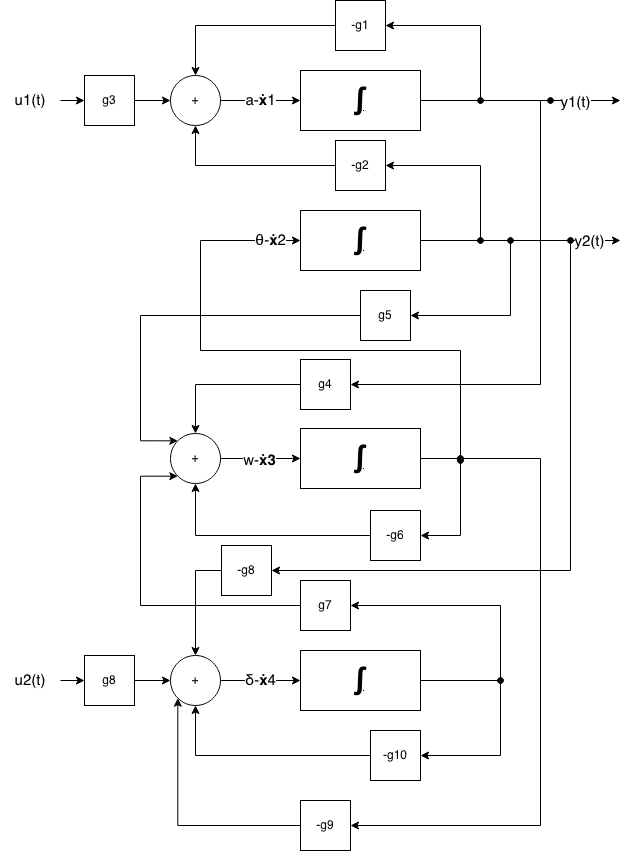
\includegraphics[width=0.78\columnwidth]{TSII - Simulation Diagram.drawio.png}
\caption{Simulation diagram of the rocket (four integrators, one per state).}\label{fig:diagrama}
\end{figure}

\begin{table}[!t]
\centering\footnotesize\setlength{\tabcolsep}{3pt}
\caption{Gains of the simulation diagram (values with $K_1=1$, $K_2=0.5$).}\label{tab:g}
\begin{tabular}{llrp{3.3cm}}
\toprule
 & Expression & Value & Path it represents\\
\midrule
$g_1$ & $(1+K_1k_a)/\tau_m$ & 1.137 & $a\to\dot a$ ($-$), engine lag and accelerometer feedback\\
$g_2$ & $c_\theta$ & 9.81 & $\theta\to\dot a$ ($-$), loss of acceleration due to gravity\\
$g_3$ & $K_1k_a/\tau_m$ & 0.070 & $u_1\to\dot a$, thrust command\\
$g_4$ & $k_\varepsilon$ & 0.12 & $a\to\dot\omega$, thrust misalignment\\
$g_5$ & $\mu$ & 1.20 & $\theta\to\dot\omega$, aerodynamic overturning (destabilizing)\\
$g_6$ & $a_d$ & 0.35 & $\omega\to\dot\omega$ ($-$), aerodynamic damping\\
$g_7$ & $k_\delta$ & 8.50 & $\delta\to\dot\omega$, nozzle effectiveness\\
$g_8$ & $K_2/\tau_s$ & 10 & $u_2\to\dot\delta$ and $\theta\to\dot\delta$ ($-$), angle command and correction\\
$g_9$ & $\lambda K_2/\tau_s$ & 6 & $\omega\to\dot\delta$ ($-$), artificial damping\\
$g_{10}$ & $1/\tau_s$ & 20 & $\delta\to\dot\delta$ ($-$), servo lag\\
\bottomrule
\end{tabular}
\end{table}

\subsubsection{State and output}
The equations take the standard state-space form
\begin{align}
\dot x&=Ax+Bu,\\
y&=Cx,\qquad C=\begin{bmatrix}1&0&0&0\\0&1&0&0\end{bmatrix},
\end{align}
a state is a quantity that, together with the others, summarizes how the rocket is right now, the four states have their own physical meaning, if $x_4=\delta$ were eliminated, the nozzle would be treated as instantaneous, the servo lag would be lost (the fast pole at $-17.3$ s$^{-1}$, which reduces the model from fourth to third order), as well as the possibility of evaluating how much the nozzle moves (the maximum nozzle deflection, one of the criteria for choosing the gains) and the possibility of analyzing servo failures (controllability).

\subsubsection{Transfer matrix}
Instead of following four internal states, $G(p)$ summarizes the rocket as a box, if input $j$ is moved, how much does output $i$ respond, there are four functions, $G_{11}$ ($u_1\to a$, the main thrust channel), $G_{22}$ ($u_2\to\theta$, the main attitude channel) and the cross ones $G_{12}$ ($u_2\to a$) and $G_{21}$ ($u_1\to\theta$), which are the mathematical version of the chain in Fig.~\ref{fig:cadena}, all of them have the same denominator, which depends on $K_1$ and $K_2$ and is obtained symbolically, with the nominal values
\begin{equation}
D(p)=p^4+21.487p^3+79.94p^2+126.76p+92.907.
\end{equation}
They share the denominator because the four states are connected (the angle affects the acceleration through gravity, and the acceleration affects the rotation through the misalignment), any input excites the same natural modes of the rocket and any output sees them, stability is therefore a property of the whole rocket and not of an isolated channel, what distinguishes each channel is the numerator, which sets how much of each mode appears in it, each channel is fourth order, with a numerator of degree 3 for $G_{11}$, 1 for $G_{21}$ and $G_{22}$, and constant for $G_{12}$.

\subsubsection{Poles, zeros and static gain}
The nominal poles are $-17.26$, $-2.09$ and $-1.07\pm1.20j$ (natural frequency 1.60 rad/s and damping 0.66 for the complex pair), all with negative real part, the rocket is stable with $(1,\,0.5)$, the zeros are also on the left ($G_{11}$: $-17.3$ and $-1.54\pm1.07j$; $G_{21}$: $-20$; $G_{22}$: $-1.14$; $G_{12}$ has none), so the system is \emph{minimum phase}, when a command is given, the output moves in the right direction from the start, it should not be confused with the negative sign of $G_{12}$, there $a$ drops immediately and stays down because of gravity, it does not change direction over time.

The pole-zero map (Fig.~\ref{fig:pz}) summarizes the dynamics, the farther to the left, the faster that mode dies out, the farther from the horizontal axis, the more it oscillates, according to the participation of each pole in the states:
\begin{itemize}
  \item $-17.26$ is the \textbf{servo} (85\% in $\delta$) and dies out in about 0.06 s, a zero of $G_{11}$ lies on top of this pole and the two cancel, so the acceleration barely sees the servo.
  \item $-1.07\pm1.20j$ is the \textbf{pitch} mode ($\theta$ 46\% and $\omega$ 33\% each), it is the slow, oscillatory mode, the one that limits how fast the rocket can be righted (the ``rebound'' of the impulse) and, therefore, \emph{limits the steering correction}.
  \item $-2.09$ mixes $\omega$, $\theta$ and $a$ (the engine and the rotation interacting), together with the previous pair it limits \emph{the acceleration correction}.
\end{itemize}
No pole is ``pure'', the coupling mixes the states.

\begin{figure}[!t]
\centering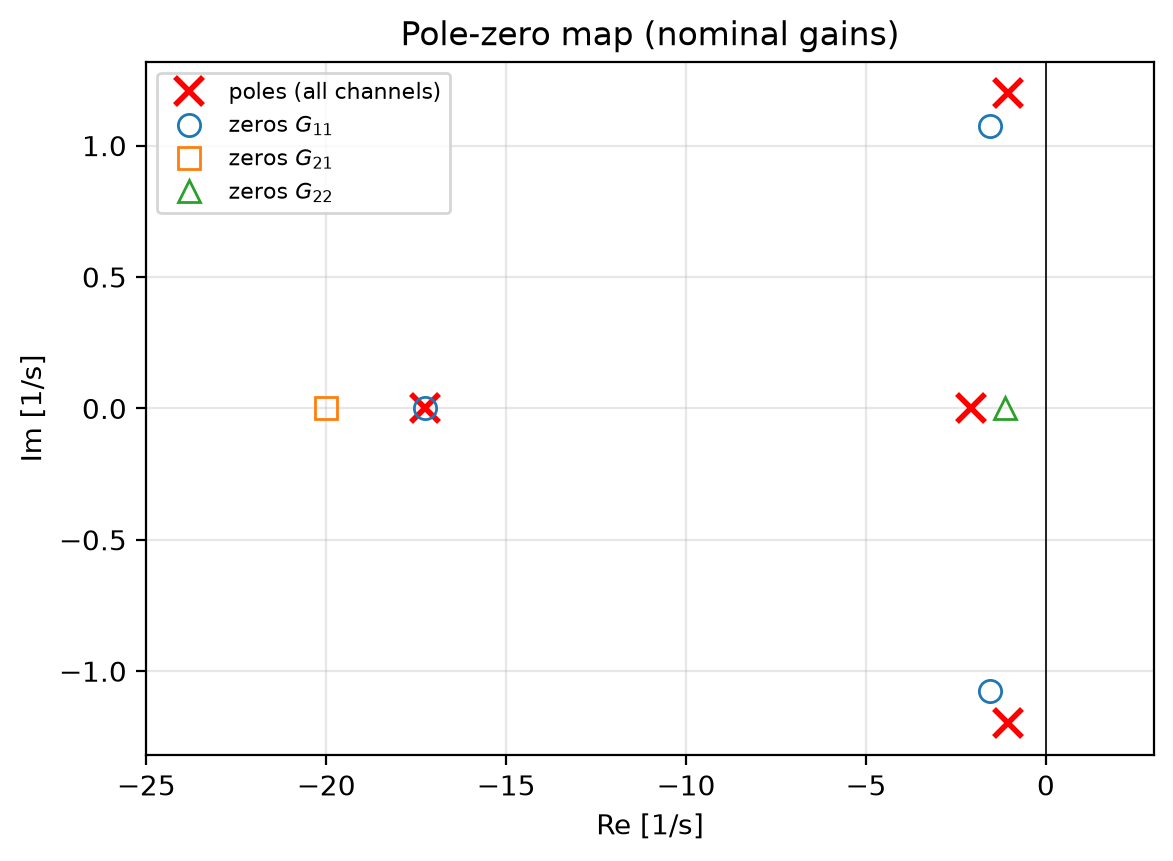
\includegraphics[width=0.85\columnwidth]{fig_polezero.png}
\caption{Poles ($\times$) and zeros ($\circ,\square,\triangle$) with the nominal gains.}\label{fig:pz}
\end{figure}

The static gain $G(0)$ (final value for a unit input) admits four physical readings,
\begin{equation}
G(0)=\begin{bmatrix}0.046&-8.98\\0.0018&1.040\end{bmatrix}.
\end{equation}
$G_{22}(0)=1.04$, asking for $5^\circ$ ends at $5.2^\circ$, almost without error, $G_{12}(0)=-8.98$, tilting the rocket 1 rad takes away almost 9 m/s$^2$ of axial acceleration, it is gravity and it was verified by hand,
\begin{equation}
G_{12}(0)=-\frac{c_\theta\tau_m\,G_{22}(0)}{1+K_1k_a}=-8.98,
\end{equation}
while $G_{11}(0)=0.046$, a unit thrust step gives a small final acceleration because $k_a$ is small, $G_{21}(0)=0.0018$, accelerating barely tilts the rocket in steady state, in terms of the test steps, 10\% thrust produces $0.459$ m/s$^2$ (about 0.05 g) and $5^\circ$ of command produces $5.20^\circ$ of pitch and a coupled acceleration of $-0.78$ m/s$^2$.


\subsection{Stability and the role of the nozzle}
A stable rocket is one that, after a hit, returns to calm, all poles with negative real part, but the rocket is aerodynamically unstable ($\mu>0$), so stability depends on the nozzle being strong enough, the characteristic polynomial
\begin{equation}
D(p)=a_4p^4+a_3p^3+a_2p^2+a_1p+a_0
\end{equation}
is a function of $K_1$ and $K_2$, and the Routh--Hurwitz criterion gives conditions on its coefficients, all of them positive and
\begin{equation}
\Delta_3=a_3a_2a_1-a_4a_1^2-a_3^2a_0>0,
\end{equation}
that guarantee stability without computing poles.

\begin{figure}[!t]
\centering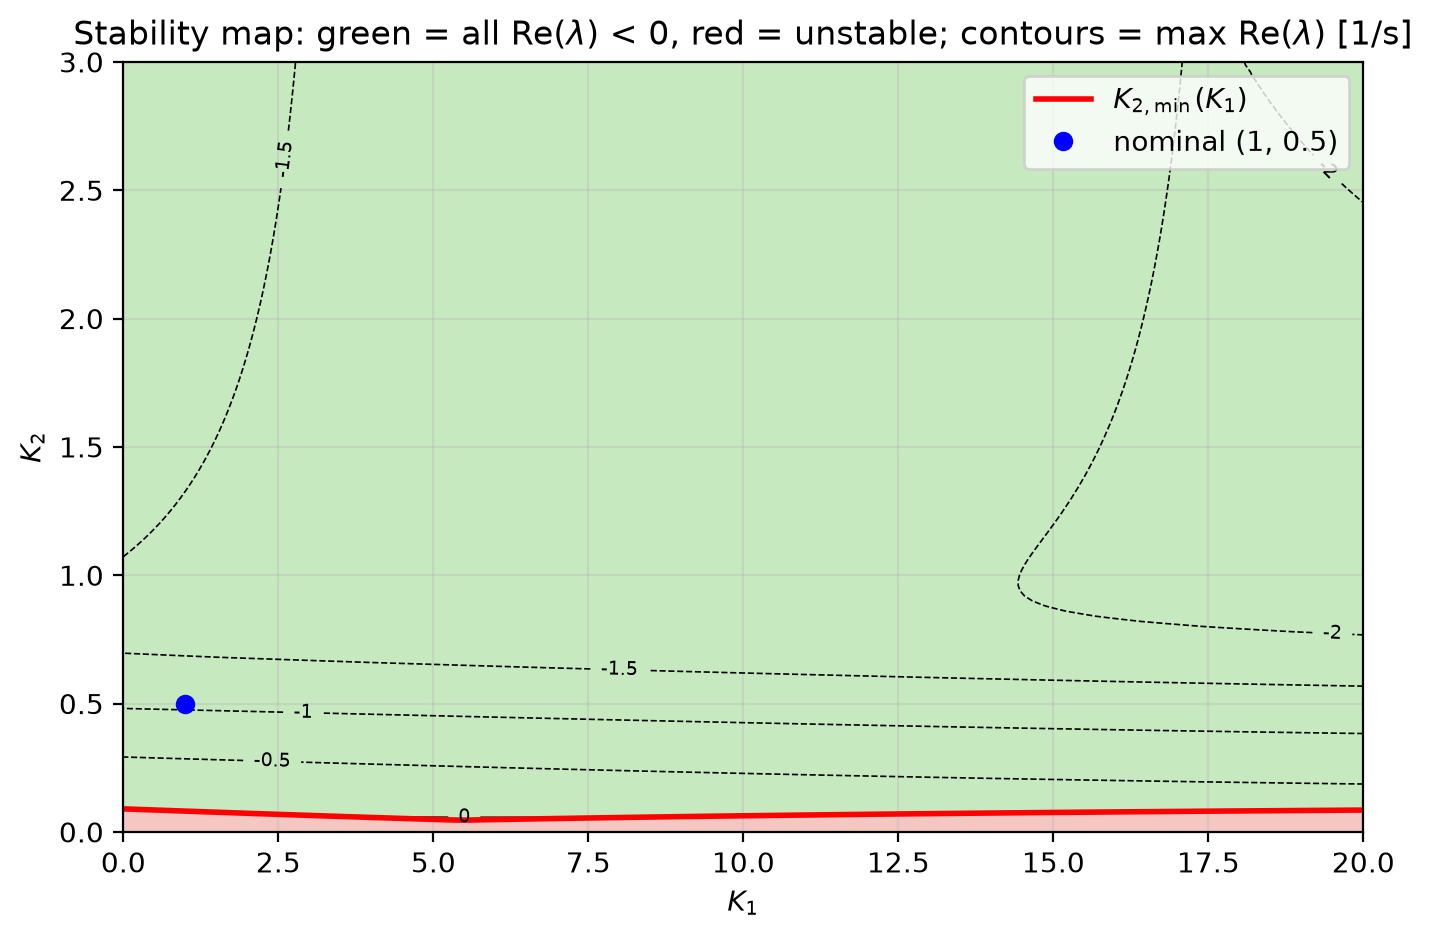
\includegraphics[width=\columnwidth]{fig_stab_map.png}
\caption{Stability map in the $(K_1,K_2)$ plane, green is stable and red is unstable, the lines are the largest $\mathrm{Re}(\lambda)$ and the red one is $K_{2,\min}(K_1)$.}\label{fig:stab}
\end{figure}

The result is in Fig.~\ref{fig:stab}, there are two parameters (the axes) and a ``stable or unstable'' answer, so a 2D map shows the whole safe region at a glance, there is a minimum $K_2$, between $0.046$ and $0.085$ for $K_1\in[0.5,\,20]$, almost the whole plane is stable, $K_2\gtrsim0.09$ is enough, the level curves (how stable the rocket is) are almost horizontal, $K_2$ rules how fast the rocket settles and $K_1$ has very little influence on stability, physically, the instability comes from $\mu$, which acts on the rotation, and the only piece that fights it is the servo, controlled by $K_2$, $K_1$ belongs to the engine channel, which was already stable, the nominal $(1,\,0.5)$ lies on the $-1$ s$^{-1}$ curve, its slowest mode dies out with a characteristic time of approximately 1 s.

\begin{figure*}[!t]
\centering
\subfloat[Acceleration $a$]{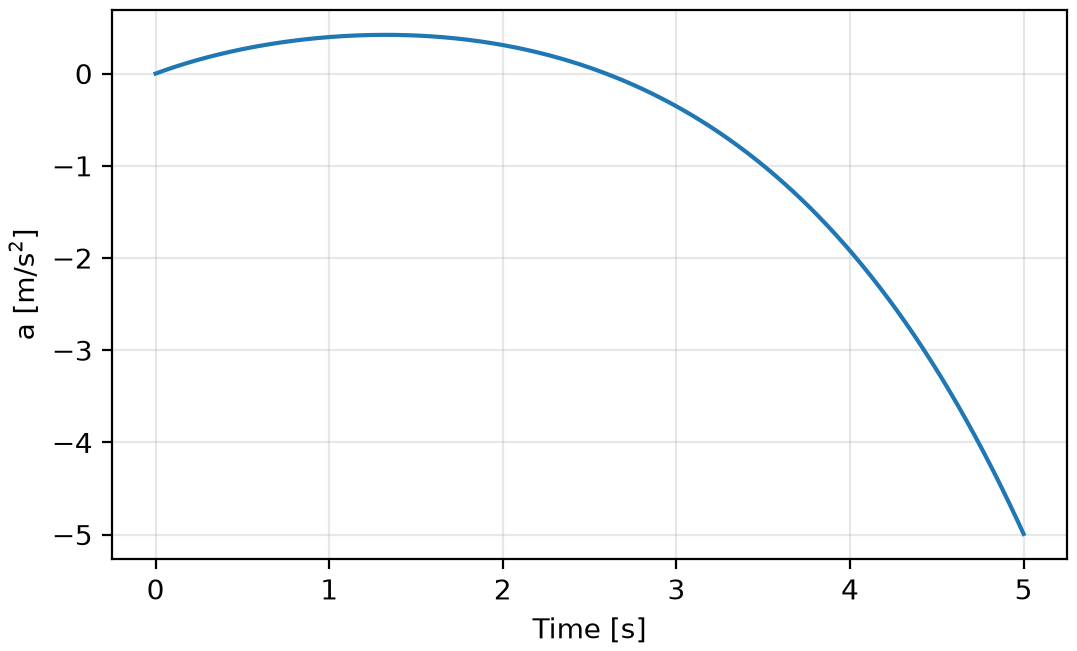
\includegraphics[width=0.4\textwidth]{en/fig_k2_0_unstable_a}}
\hfill
\subfloat[Angles $\theta$ and $\delta$]{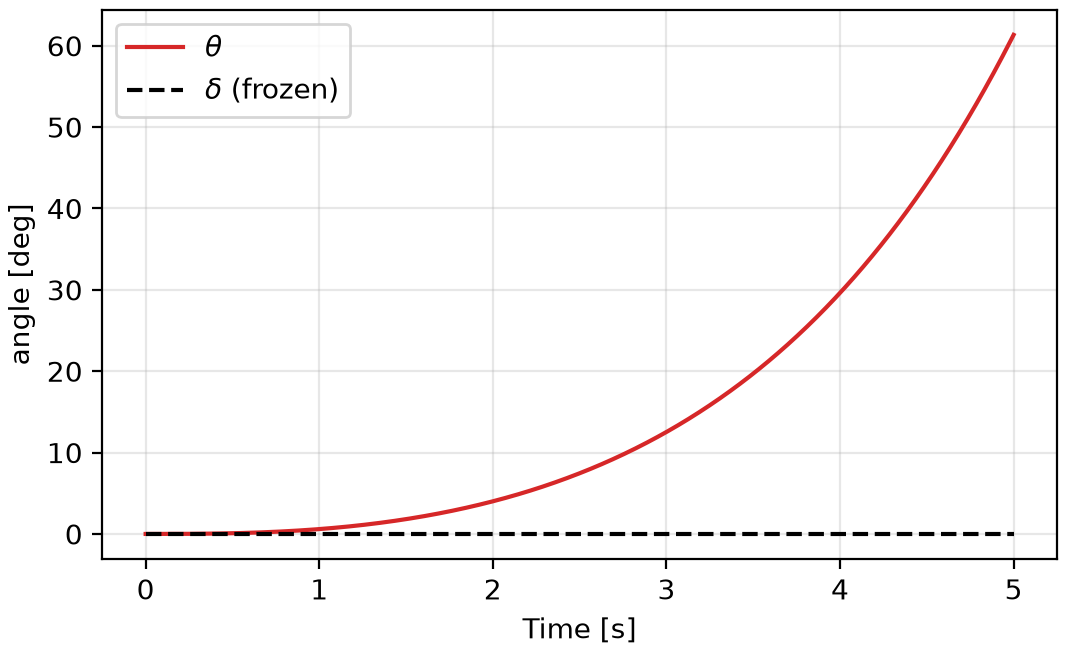
\includegraphics[width=0.4\textwidth]{en/fig_k2_0_unstable_b}}
\caption{Case $K_2=0$ with a 10\% thrust step, $\theta$ grows and $\delta$ stays frozen at 0.}\label{fig:k20}
\end{figure*}

With $K_2=0$ the servo is disconnected and the nozzle never moves, a pole appears at $+0.557$ s$^{-1}$, so the angle is multiplied by $e^{0.557}\approx1.75$ every second (Fig.~\ref{fig:k20}), $\theta$ rises to about $60^\circ$ in 5 s, and the acceleration, which starts rising because the engine does respond to $u_1$, becomes negative because the growing tilt takes away acceleration through $-c_\theta\theta$, without steering, the air (which acts through $\mu$) overturns the rocket.


\subsection{Response to test signals and effect of the gains}
To get to know a rocket it is ``hit'' in different ways and its reaction is observed, three signals were used (with unit input, only for the linear analysis), a \emph{pulse} $H(t)-H(t-5)$, which is a maneuver that turns on for 5 s and turns off, a \emph{sinusoid} $\sin t$, like a periodic vibration or air currents, and an \emph{impulse} $K\delta(t)$, a gust, each one was applied to $u_1$ alone, to $u_2$ alone and to both, to separate the cause, $y(t)=[a,\theta]$ is always plotted against time, because it is what an engineer would see in the telemetry.

\begin{figure*}[!t]
\centering
\subfloat[$u_1$ only]{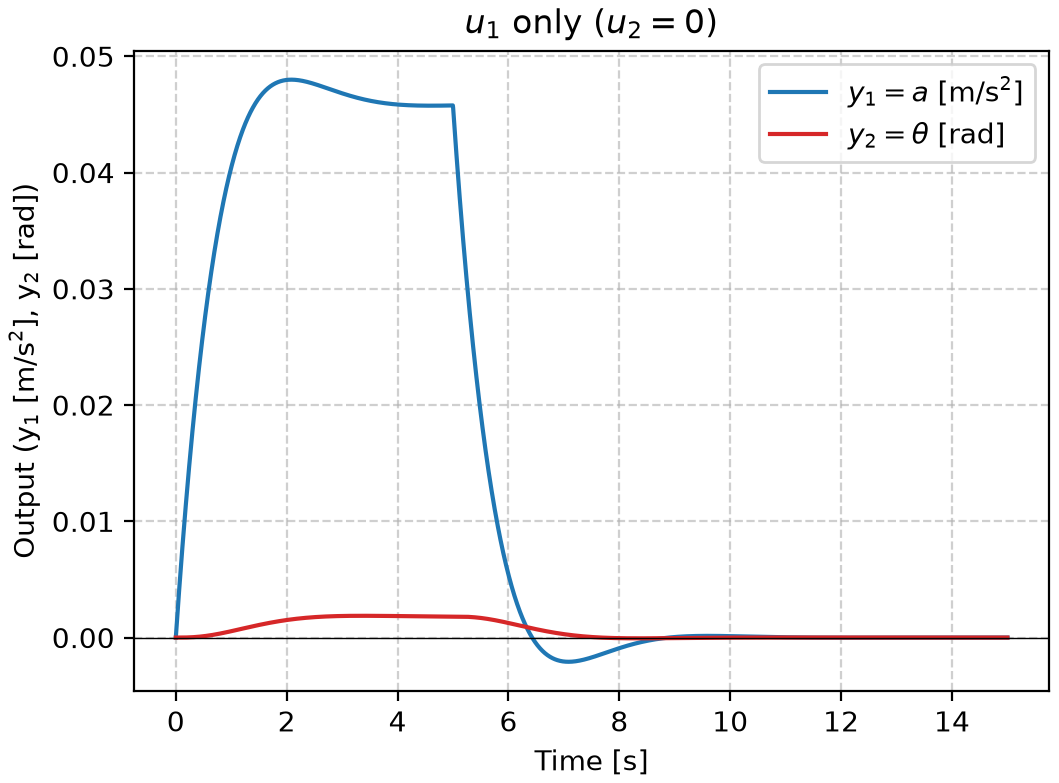
\includegraphics[width=0.32\textwidth]{en/fig_q7_pulse_a}}
\hfill
\subfloat[$u_2$ only]{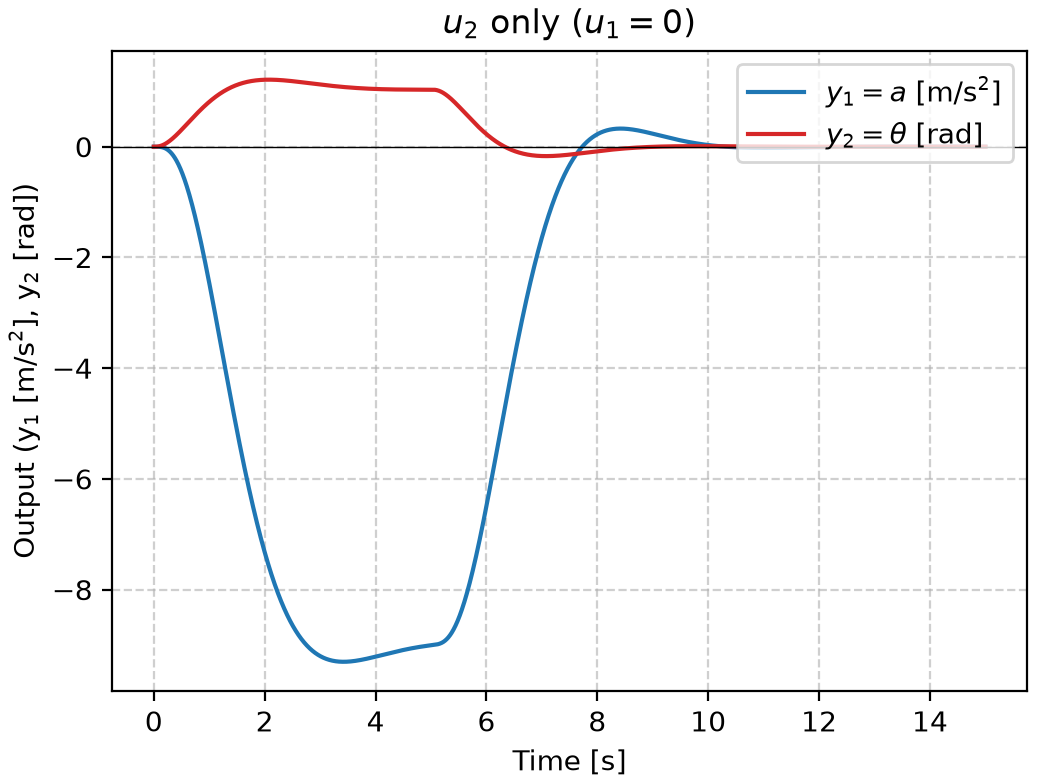
\includegraphics[width=0.32\textwidth]{en/fig_q7_pulse_b}}
\hfill
\subfloat[$u_1$ and $u_2$ together]{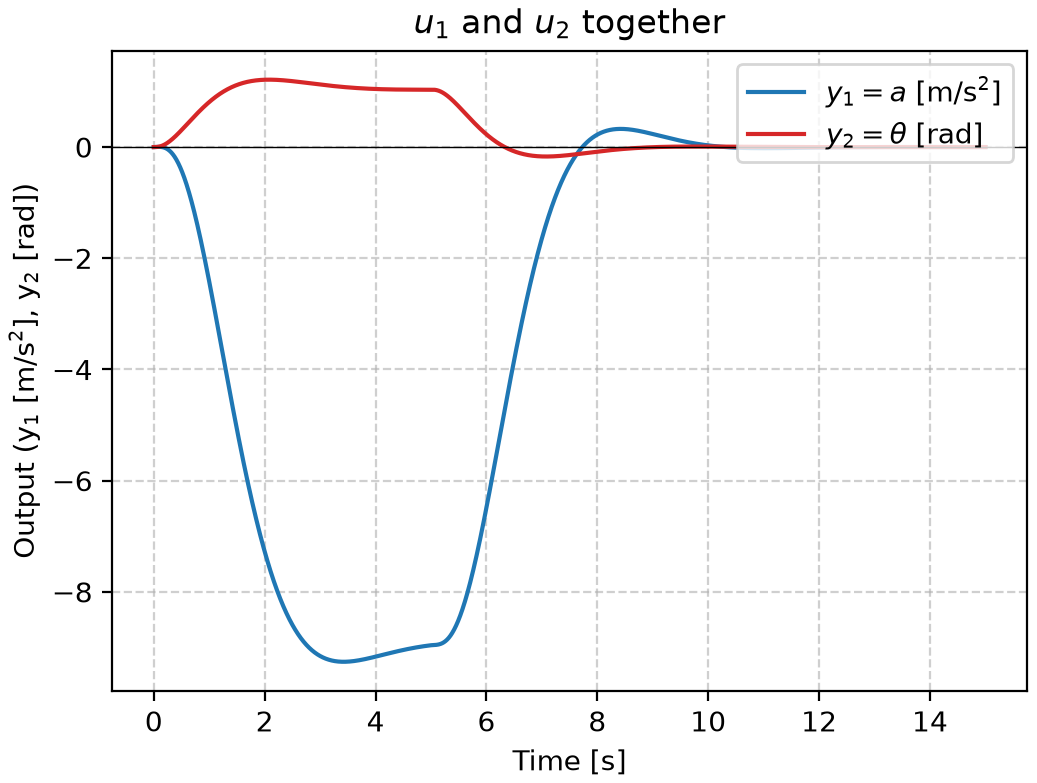
\includegraphics[width=0.32\textwidth]{en/fig_q7_pulse_c}}
\caption{Response to the 5 s rectangular pulse.}\label{fig:pulse}
\end{figure*}

\subsubsection{Pulse}
With $u_1$ alone, $a$ rises to about $0.048$ m/s$^2$ in 2 s and stays there while the pulse lasts, while $\theta$ barely moves ($0.002$ rad), when the pulse ends, $a$ returns to zero in about 2 s, with $u_2$, $\theta$ rises to $1.1$ rad and stays near 1 rad, while $a$ \emph{drops} to about $-9$ m/s$^2$, it is the gravity coupling, $G_{12}(0)\approx-8.98$, when the pulse ends the servo and the controller right the rocket and $a$ rebounds slightly ($+0.3$) before settling, the values at which the curves stay during the pulse are the static gain $G(0)$, and all of them return to zero after the pulse (stability).

\begin{figure*}[!t]
\centering
\subfloat[$u_1$ only]{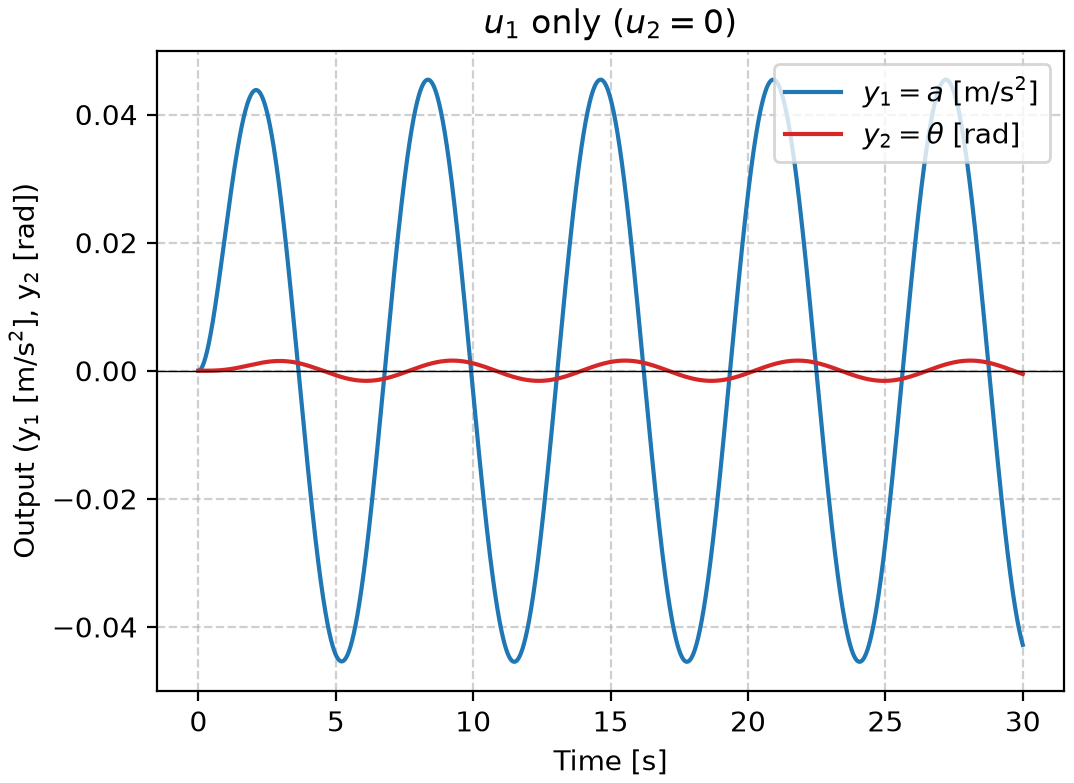
\includegraphics[width=0.32\textwidth]{en/fig_q7_sine_a}}
\hfill
\subfloat[$u_2$ only]{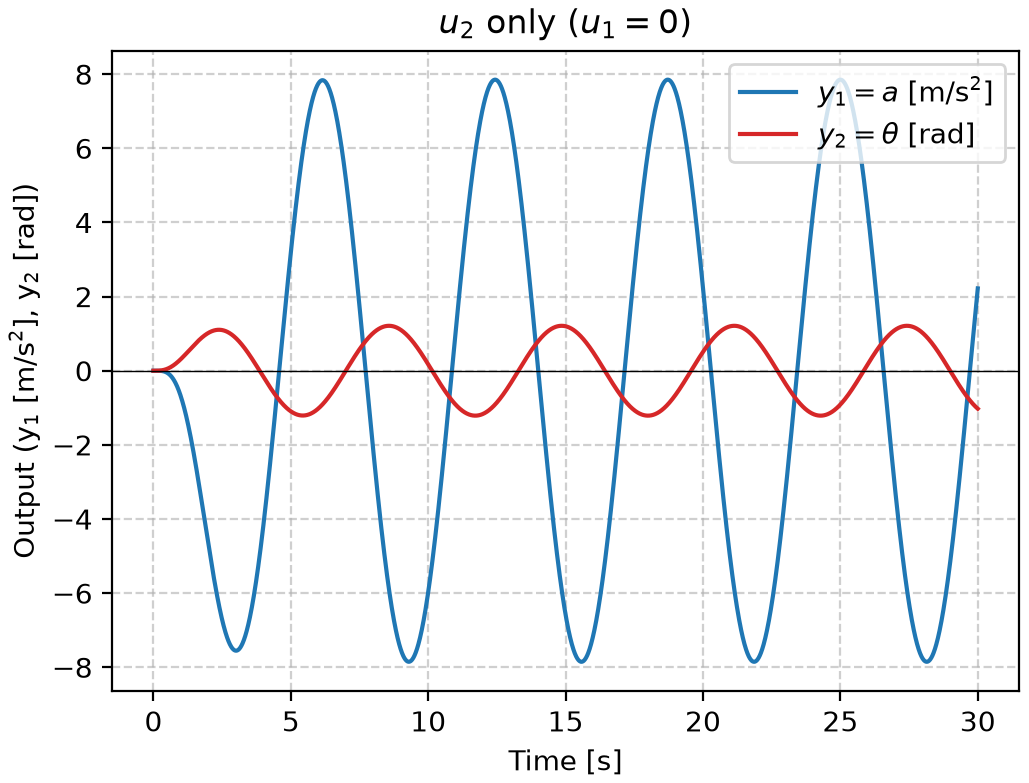
\includegraphics[width=0.32\textwidth]{en/fig_q7_sine_b}}
\hfill
\subfloat[$u_1$ and $u_2$ together]{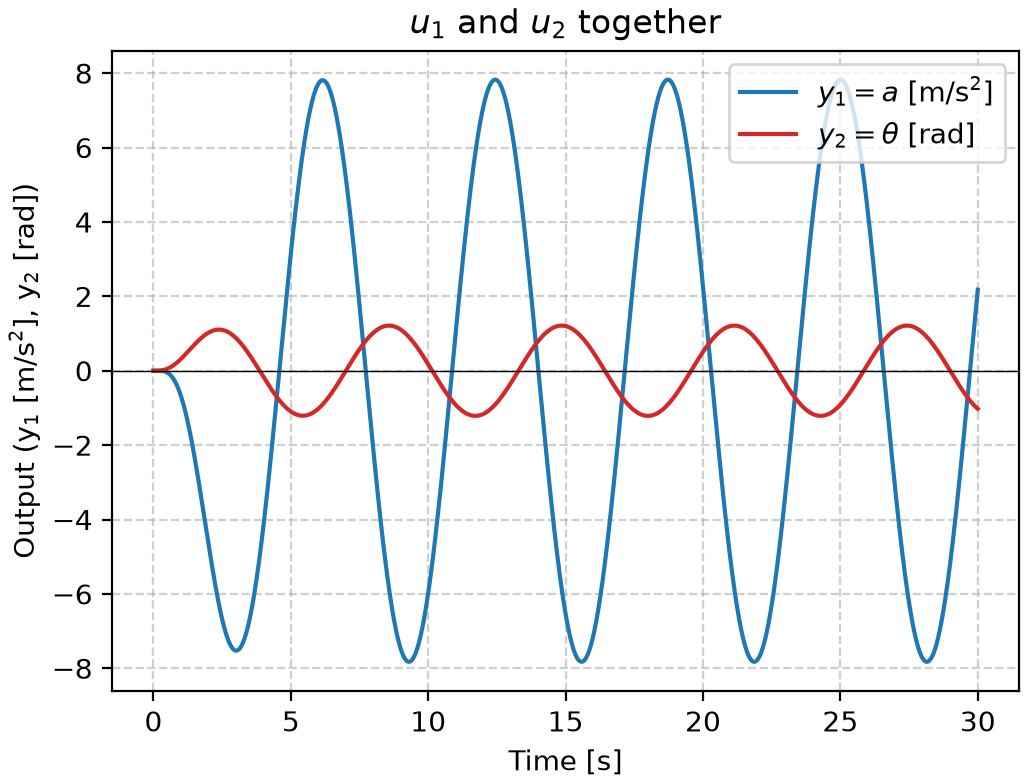
\includegraphics[width=0.32\textwidth]{en/fig_q7_sine_c}}
\caption{Response to the sinusoidal input $\sin t$ ($\omega=1$ rad/s).}\label{fig:sine}
\end{figure*}

\subsubsection{Sinusoid}
After a short transient the outputs oscillate at the same frequency as the input (period $2\pi\approx6.3$ s) with constant amplitude, $a$ of $\pm0.045$ from $u_1$, $a\approx\pm7.8$ and $\theta\approx\pm1.2$ from $u_2$, it is the basis of the frequency response, a stable system responds to a sinusoid with another sinusoid of the same frequency, with a different amplitude and phase, at 1 rad/s the amplitudes are approximately the static gains, because 1 rad/s is within the bandwidth of the rocket, which is around 2 rad/s.

\begin{figure*}[!t]
\centering
\subfloat[$u_1$ only]{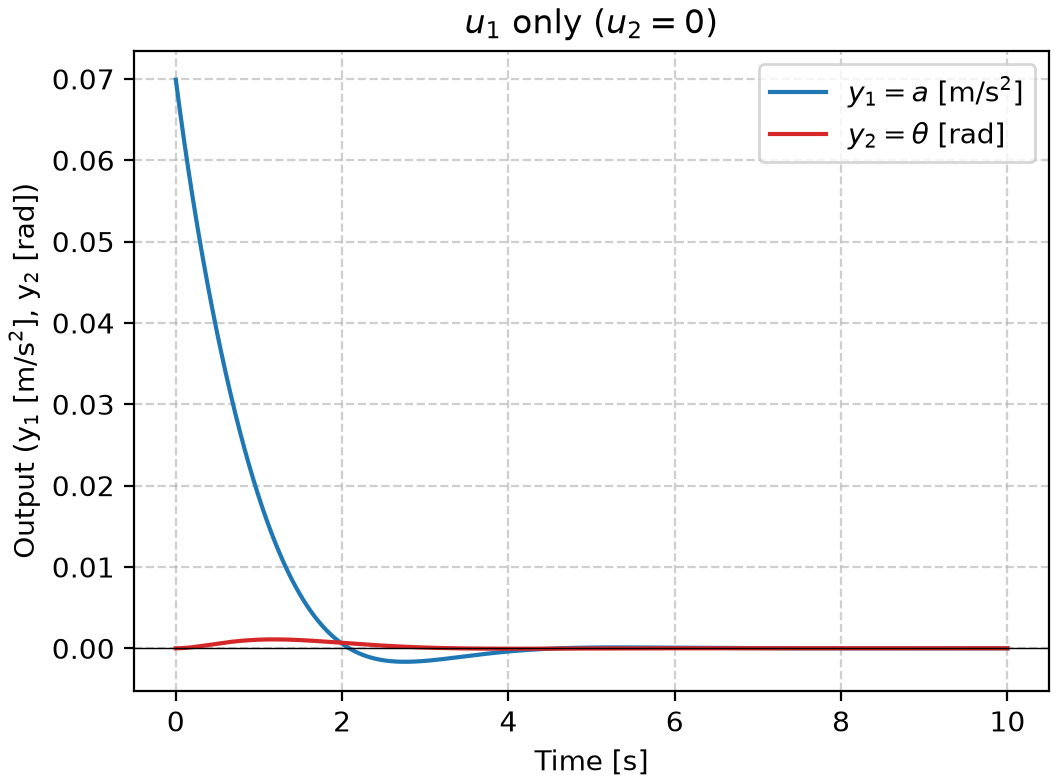
\includegraphics[width=0.32\textwidth]{en/fig_q7_impulse_a}}
\hfill
\subfloat[$u_2$ only]{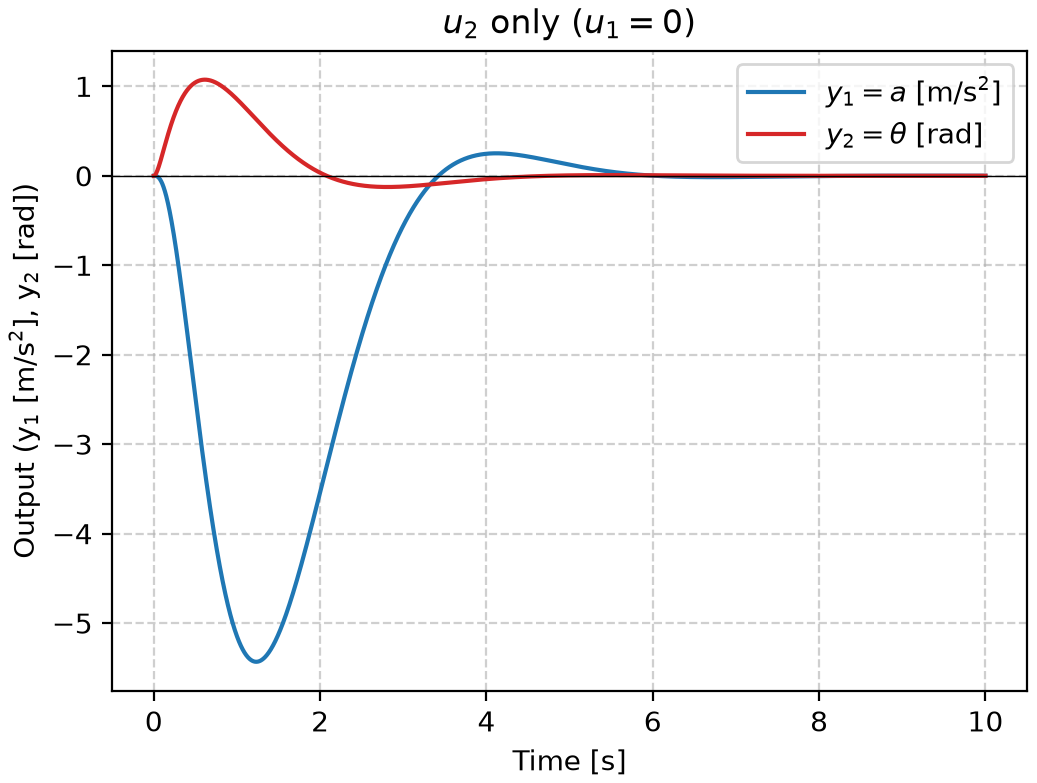
\includegraphics[width=0.32\textwidth]{en/fig_q7_impulse_b}}
\hfill
\subfloat[$u_1$ and $u_2$ together]{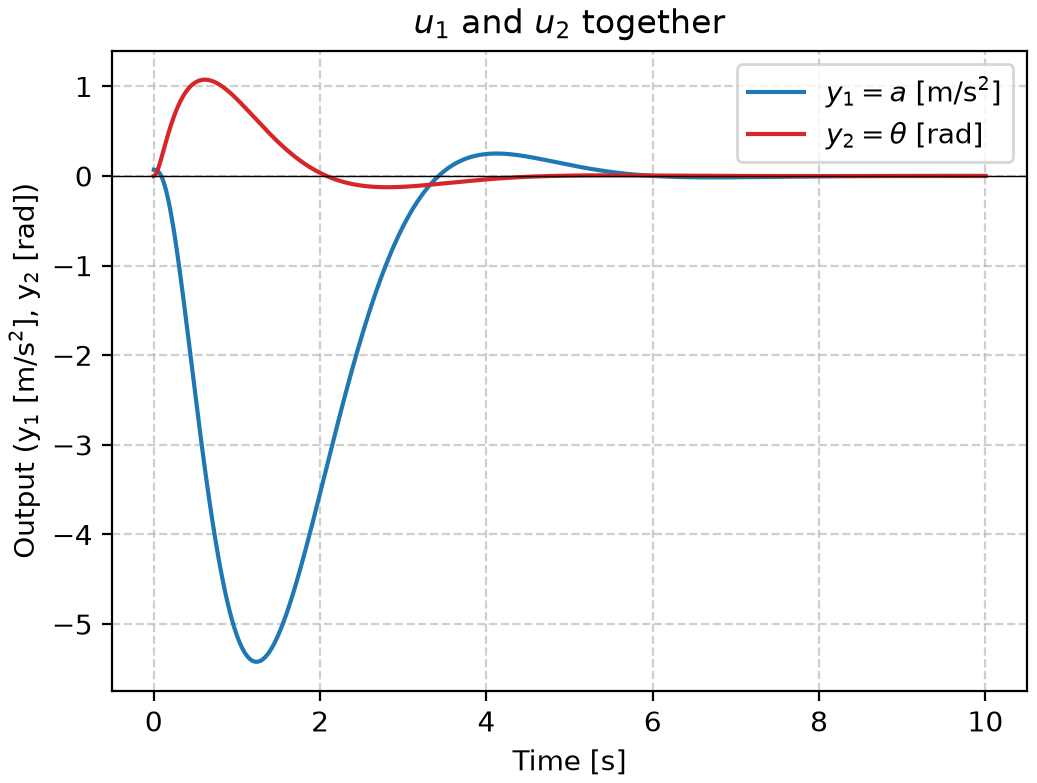
\includegraphics[width=0.32\textwidth]{en/fig_q7_impulse_c}}
\caption{Response to the impulse (gust) $K\delta(t)$ with $K=1$.}\label{fig:impulse}
\end{figure*}

\subsubsection{Impulse}
A gust dies out by itself in 5--6 s (Fig.~\ref{fig:impulse}), with $u_2$, $\theta$ rises to $1.1$ rad in 0.6 s and $a$ falls to $-5.4$ m/s$^2$ in 1.2 s, both return to zero with a soft rebound, an impulse excites all the modes at once, and the way it dies out is the fingerprint of the poles, the envelope decays as $e^{-1.07t}$ (slow poles $-1.07\pm1.20j$) and the rebound is the effect of their imaginary part, the fast pole $-17.3$ dies out in a tenth of a second and is barely seen, with $u_1$ alone, the curve of $a$ starts at $0.07$ m/s$^2$ instantaneously, which is $K_1k_a/\tau_m$, $u_1$ enters directly into the state $a$ (the only channel with an initial jump, since the others have three or four links).

\begin{figure*}[!t]
\centering
\subfloat[$\theta$ against $K_2$, $5^\circ$ step in $u_2$]{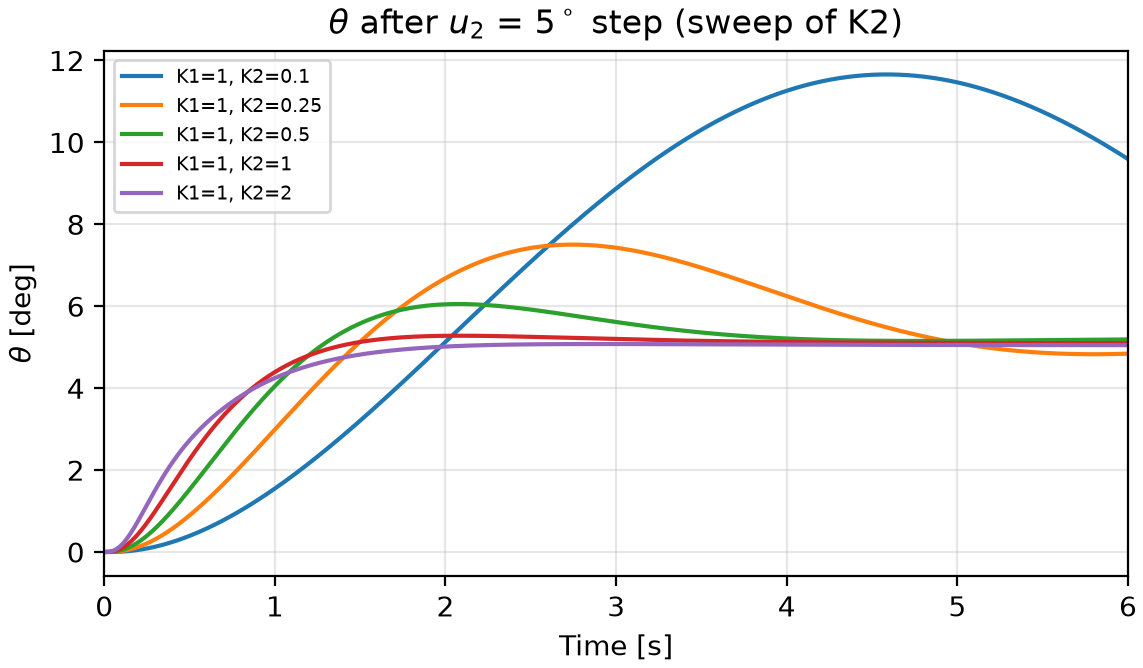
\includegraphics[width=0.4\textwidth]{en/fig_q7_gain_sweep_a}}
\hfill
\subfloat[$a$ against $K_2$, 10\% step in $u_1$]{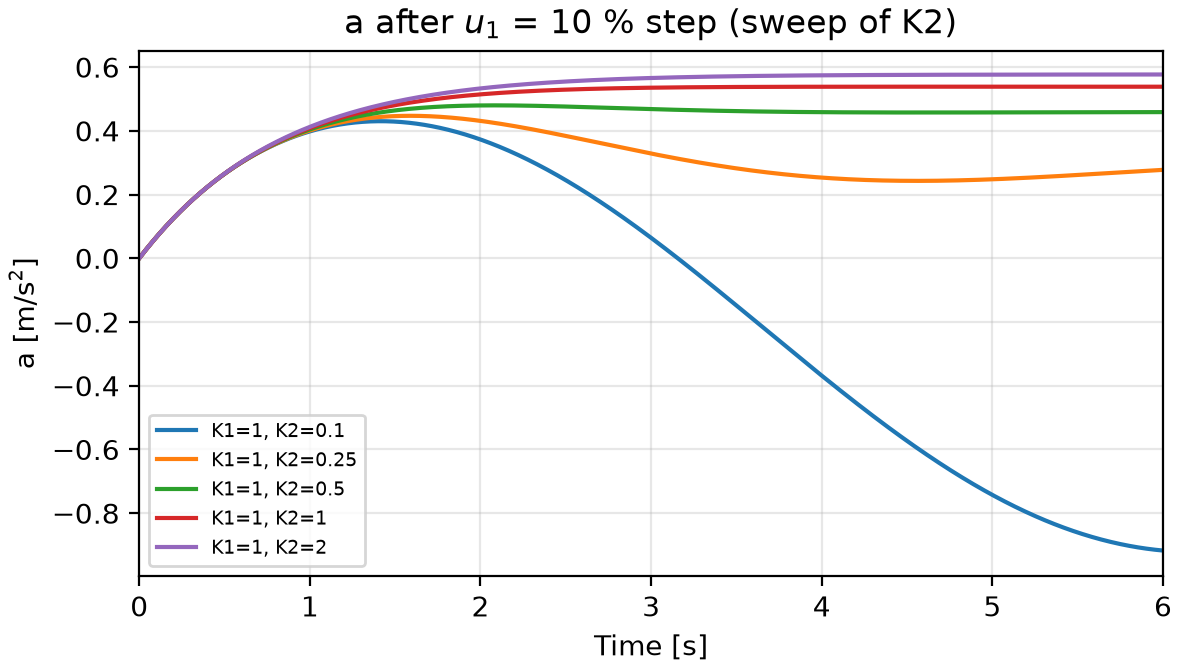
\includegraphics[width=0.4\textwidth]{en/fig_q7_gain_sweep_b}}
\\
\subfloat[$\theta$ against $K_1$, $5^\circ$ step in $u_2$]{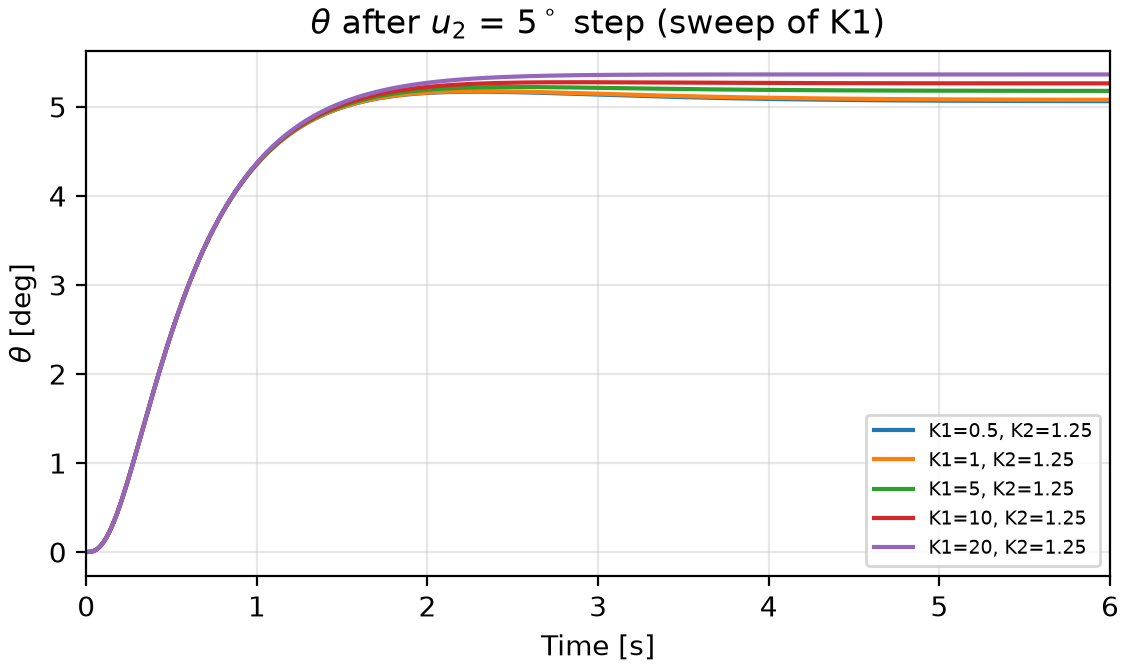
\includegraphics[width=0.4\textwidth]{en/fig_q7_gain_sweep_c}}
\hfill
\subfloat[$a$ against $K_1$, 10\% step in $u_1$]{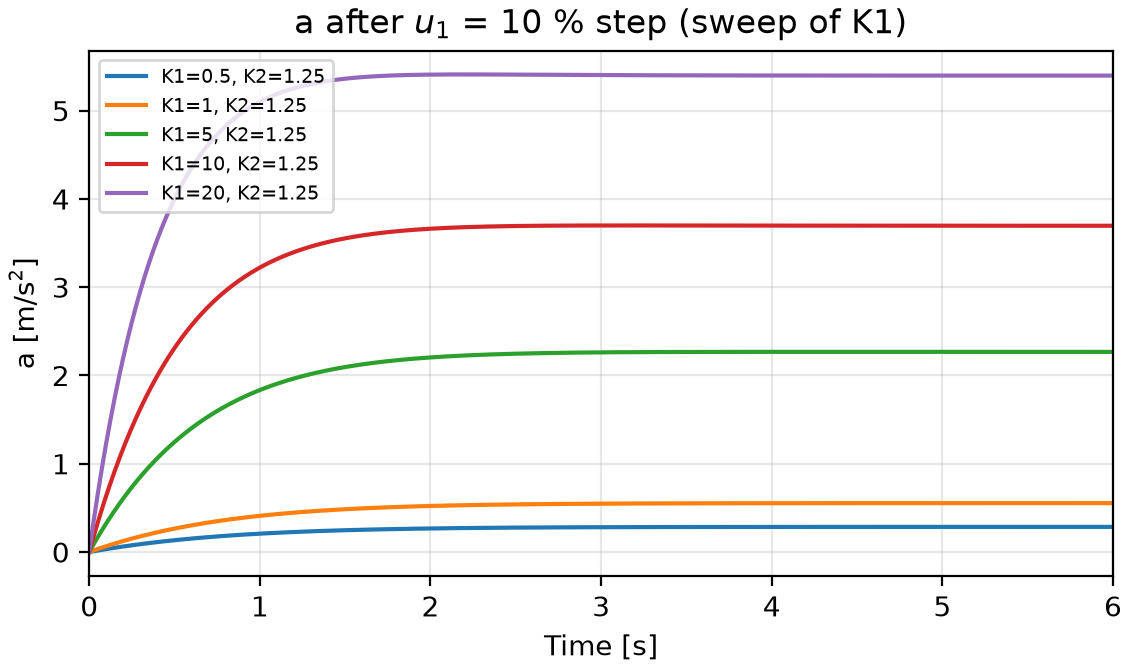
\includegraphics[width=0.4\textwidth]{en/fig_q7_gain_sweep_d}}
\caption{Effect of the gains on speed and stability, sweep of $K_2$ with $K_1=1$ in (a) and (b), sweep of $K_1$ with $K_2=1.25$ in (c) and (d).}\label{fig:sweep}
\end{figure*}

\subsubsection{Effect of the gains}
The fastest way to see the effect of a knob is to overlay one curve per gain (Fig.~\ref{fig:sweep}), in (a), with a $5^\circ$ step in $u_2$, with $K_2=0.1$ the rocket overshoots up to $11.7^\circ$ and takes more than 6 s to settle (the nozzle has almost no strength to brake), with $K_2=0.25$ it reaches $7.5^\circ$ (50\% overshoot), with $K_2\ge1$ it rises fast and clean, in (c) and (d), with $K_2=1.25$ fixed, $\theta$ barely depends on $K_1$, but the final acceleration does, from $0.3$ m/s$^2$ with $K_1=0.5$ to $5.4$ m/s$^2$ with $K_1=20$ for the same 10\% thrust, each gain has its own job, $K_2$ governs the attitude (speed and damping of the rotation) and $K_1$ governs how much acceleration is obtained with the thrust command.


\subsection{Coupling between channels}
\subsubsection{How much the channels are coupled}
Since $a$ and $\theta$ cannot be compared directly (m/s$^2$ against rad), each cross deviation is measured with respect to the main output of the other channel, with steps of $u_1=10\%$ and $u_2=5^\circ$ (Fig.~\ref{fig:coupling}), with the nominal gains,
\begin{itemize}
  \item a step in $u_2$ takes $\theta$ to $5.20^\circ$, but the acceleration drops to $-0.81$ m/s$^2$ and stays at $-0.78$, the tilt takes away almost 0.8 m/s$^2$, compared with the $0.459$ m/s$^2$ that 10\% thrust gives, the coupling $u_2\to a$ is \textbf{177\%}, tilting the rocket takes away more acceleration than the thrust gives it.
  \item a step in $u_1$ takes $a$ to $0.459$ m/s$^2$ and deflects $\theta$ up to $1.07^\circ$ (it ends at $1.03^\circ$, because of $k_\varepsilon$), compared with the $5.20^\circ$ of $u_2$, it is \textbf{20.6\%}.
\end{itemize}
The coupling is asymmetric and the most severe one is $u_2\to a$, gravity ($c_\theta=9.81$, large) makes that path strong, and $k_\varepsilon=0.12$ (small) makes the other weak, with the nominal gains, the attitude channel contaminates the acceleration channel.

\begin{figure*}[!t]
\centering
\subfloat[$5^\circ$ step in $u_2$]{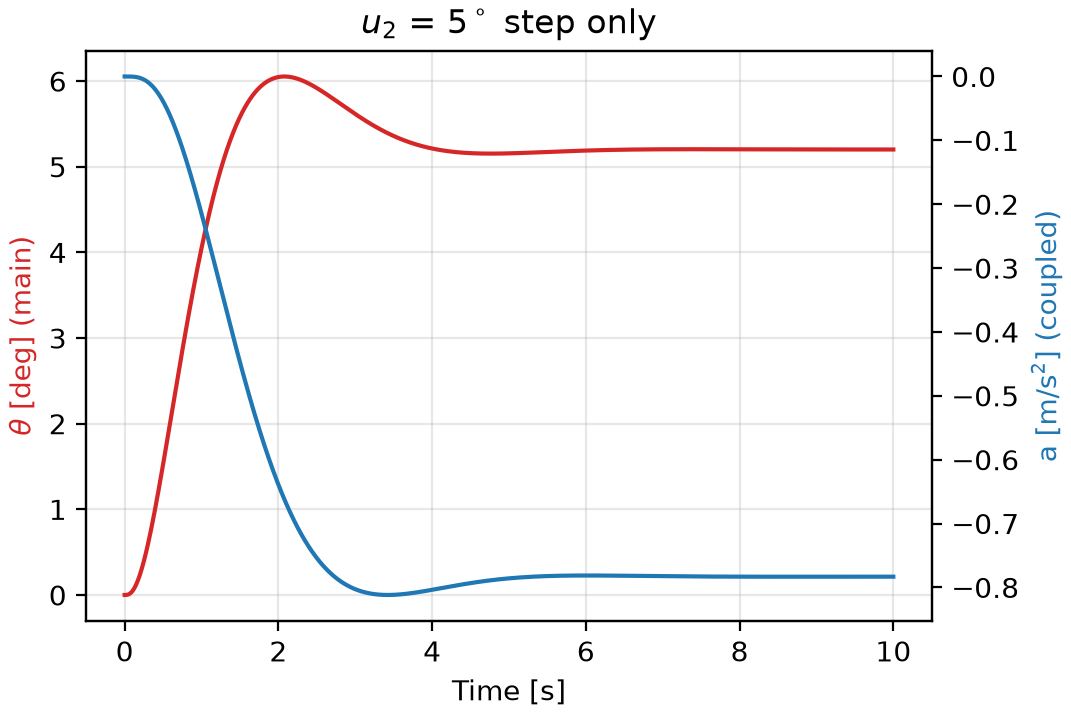
\includegraphics[width=0.4\textwidth]{en/fig_coupling_a}}
\hfill
\subfloat[10\% step in $u_1$]{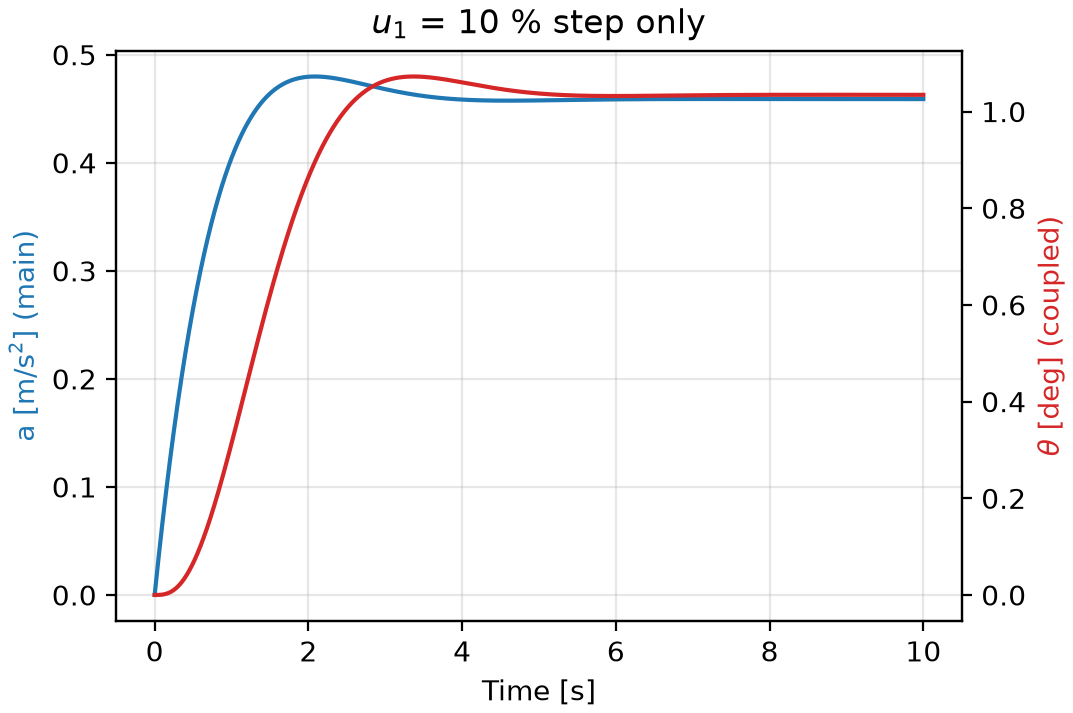
\includegraphics[width=0.4\textwidth]{en/fig_coupling_b}}
\caption{Two steps, each one with the main output and the coupled one on two vertical axes.}\label{fig:coupling}
\end{figure*}

\subsubsection{Dependence on the gains}
The percentages depend on the gains through $G(0)$ (Table~\ref{tab:acople}), raising $K_1$ from 1 to 10 multiplies $G_{11}(0)$ by 7 and reduces $u_2\to a$ from 177\% to 18\%, but the larger thrust tilts the rocket more through $k_\varepsilon$ and $u_1\to\theta$ rises to 133\%, raising $K_2$ to $1.3$ makes the nozzle hold the tilt better and $u_1\to\theta$ drops to 7.6\%, no extreme lowers both at the same time, an intermediate pair, $(4.5,\,1.3)$, gives 30.5\% and 28.3\%.

\begin{table}[!t]
\centering\footnotesize\setlength{\tabcolsep}{2.5pt}
\caption{Coupling for different gains.}\label{tab:acople}
\begin{tabular}{rr|rrrr|rr}
\toprule
$K_1$ & $K_2$ & $G_{11}$ & $G_{12}$ & $G_{21}$ & $G_{22}$ & $u_2\!\to\! a$ & $u_1\!\to\!\theta$\\
 & & \multicolumn{4}{c|}{(at $p=0$)} & [\%] & [\%]\\
\midrule
1 & 0.5 & 0.046 & $-8.98$ & 0.0018 & 1.040 & 176.9 & 20.6\\
10 & 0.5 & 0.325 & $-6.35$ & 0.0128 & 1.144 & 17.7 & 132.5\\
1 & 1.3 & 0.056 & $-8.76$ & 0.0007 & 1.015 & 137.4 & 7.6\\
4.5 & 1.3 & 0.210 & $-7.33$ & 0.0026 & 1.033 & 30.5 & 28.3\\
\bottomrule
\end{tabular}
\end{table}

\subsubsection{Frequency response}
To see how the coupling depends on the speed of the maneuver, we move on to the frequency response.

\begin{figure*}[!t]
\centering
\subfloat[$G_{11}$ ($u_1\to a$)]{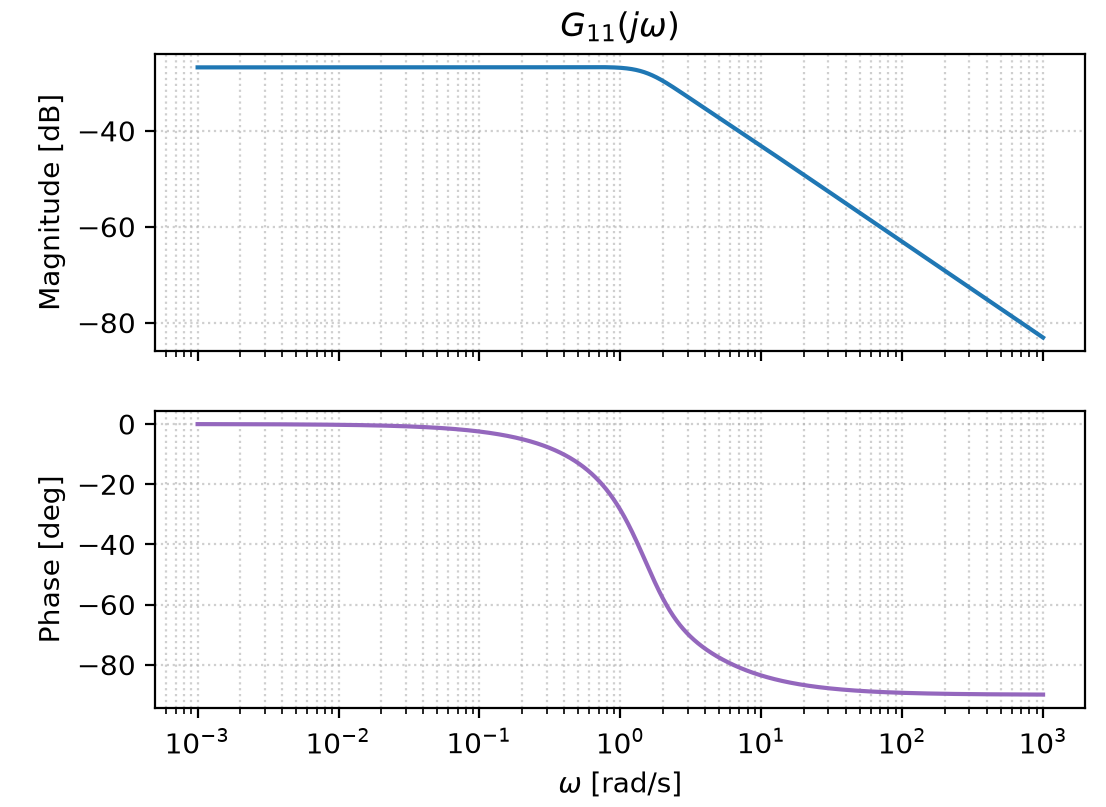
\includegraphics[width=0.4\textwidth]{en/fig_bode_2x2_a}}
\hfill
\subfloat[$G_{12}$ ($u_2\to a$)]{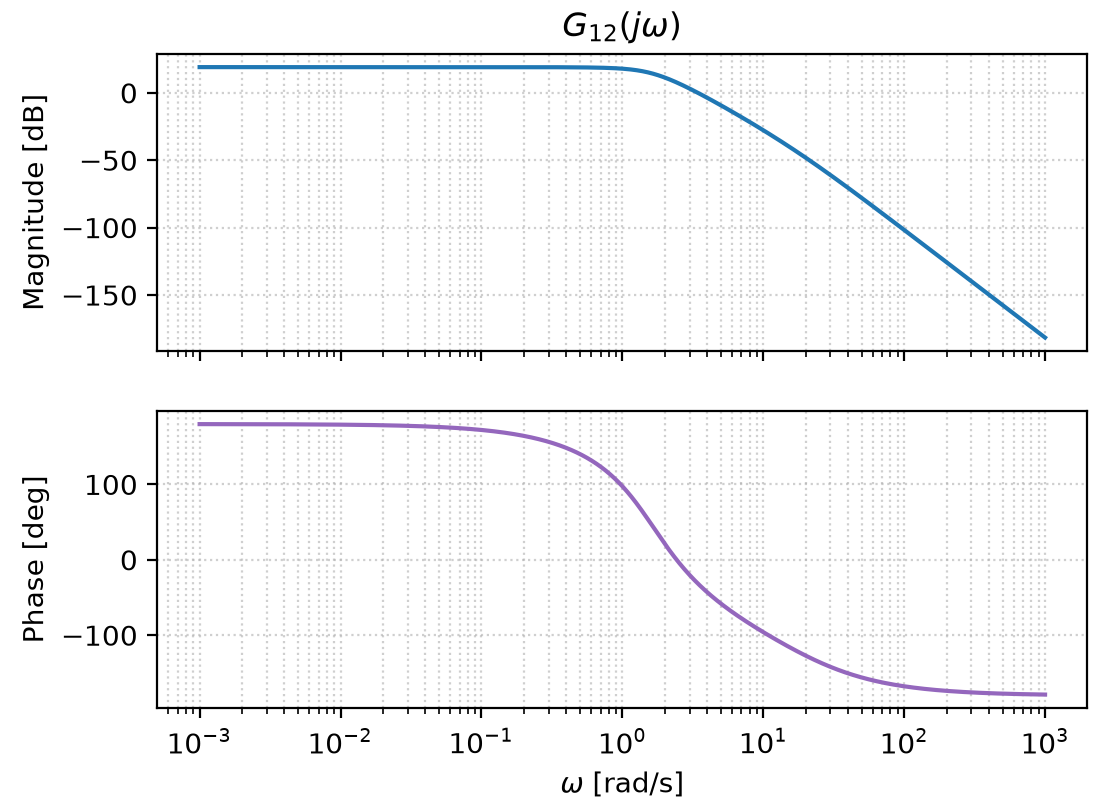
\includegraphics[width=0.4\textwidth]{en/fig_bode_2x2_b}}
\\
\subfloat[$G_{21}$ ($u_1\to\theta$)]{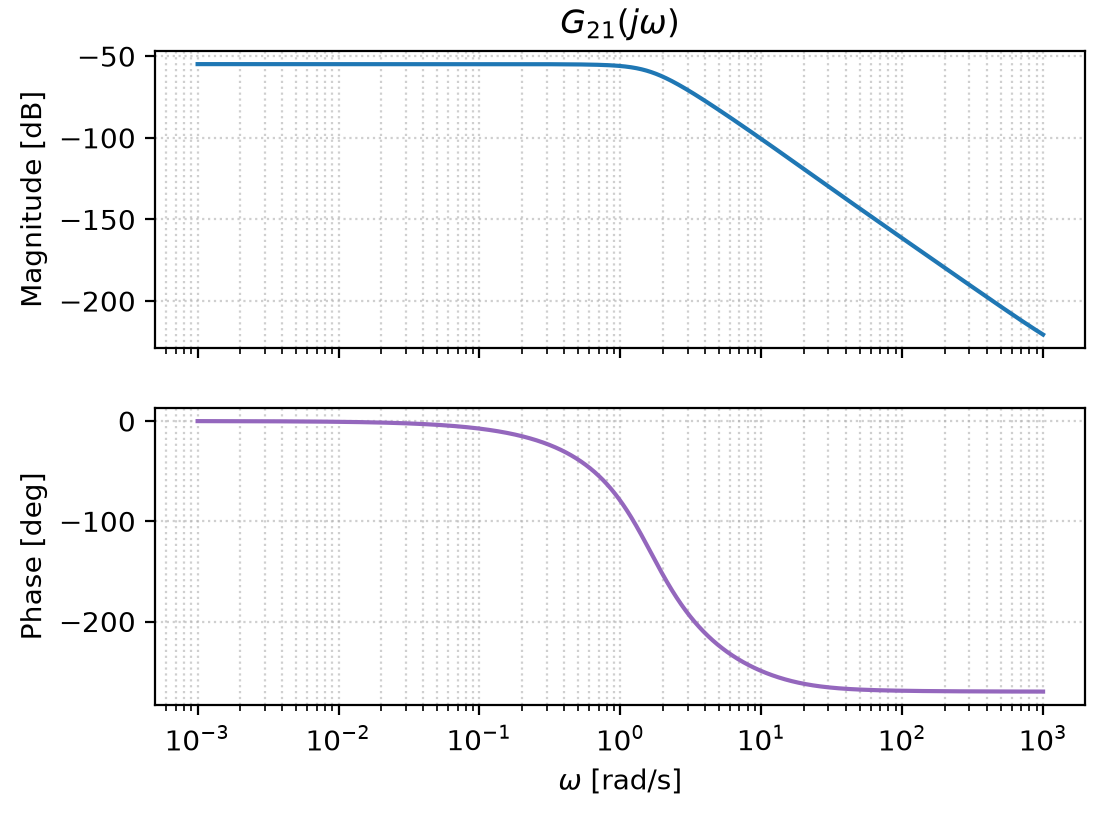
\includegraphics[width=0.4\textwidth]{en/fig_bode_2x2_c}}
\hfill
\subfloat[$G_{22}$ ($u_2\to\theta$)]{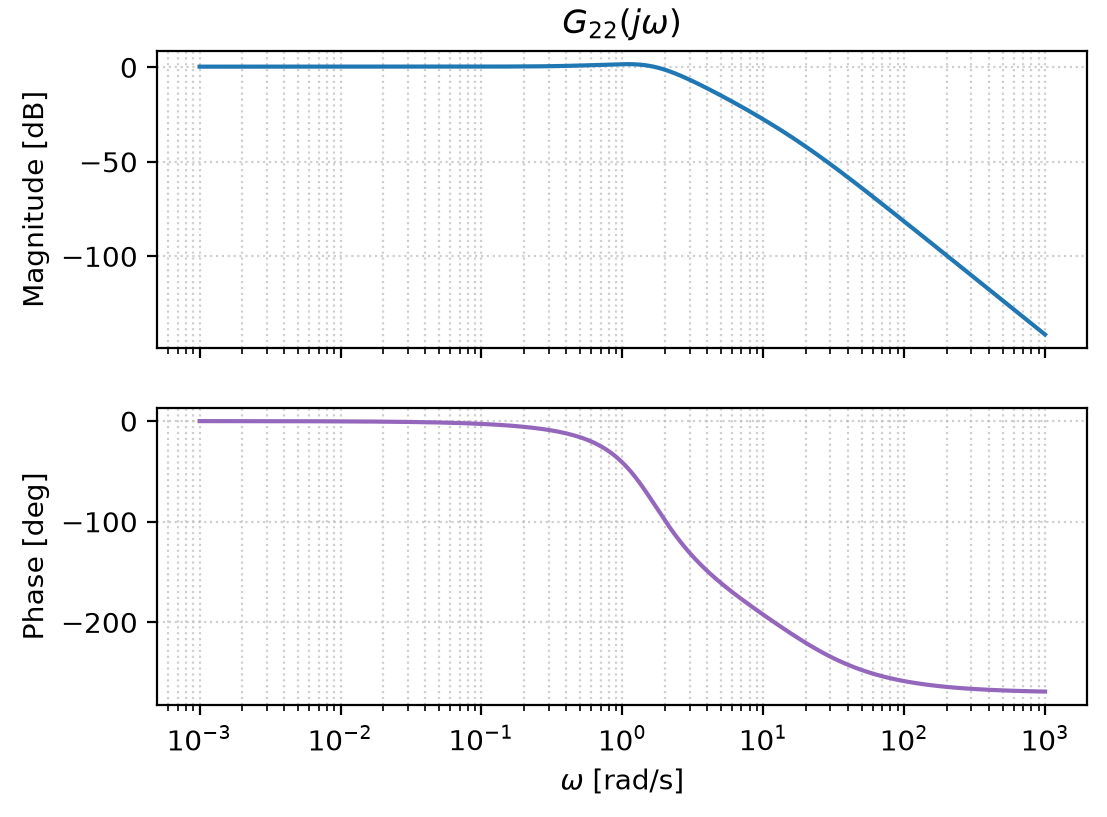
\includegraphics[width=0.4\textwidth]{en/fig_bode_2x2_d}}
\caption{Bode diagram of the four channels with $(K_1,K_2)=(1,\,0.5)$, magnitude on top and phase below in each panel.}\label{fig:bode}
\end{figure*}

The Bode diagram (Fig.~\ref{fig:bode}) shows, for each channel, the gain in decibels (dB, $-20$ dB is a tenth, $0$ dB is equal, $+20$ dB is ten times) and the phase lag against frequency, on a logarithmic scale because it spans six orders of magnitude, all the channels have a ``plateau'' at low frequency, which is $G(0)$, $-27$ dB ($0.046$) in $G_{11}$, $0$ dB in $G_{22}$ (the rocket follows the command, with a small hump near 1--2 rad/s), $+19$ dB ($8.98$) in $G_{12}$ with an initial phase of $180^\circ$ (it is the negative sign, tilting subtracts acceleration) and $-55$ dB ($0.0018$) in $G_{21}$, at high frequencies the magnitude falls with a slope of $-20\,r$ dB/decade, where $r$ is the \emph{relative degree} (number of poles minus number of zeros), $G_{11}$ has 4 poles and 3 zeros ($r=1$), $G_{21}$ and $G_{22}$ have 4 poles and 1 zero ($r=3$) and $G_{12}$ has 4 poles and no zeros ($r=4$), physically, each pole without a zero to compensate it is one more link between the command and the output (a lag of the engine, of the servo or of the rotation) that at high frequencies attenuates 20 dB per decade and adds $-90^\circ$ of phase, that is why the final phase tends to $-90^\circ$ in $G_{11}$ and to $-270^\circ$ in $G_{21}$ and $G_{22}$, the measured slopes, $-20.0$, $-79.9$, $-60.0$ and $-59.9$ dB/decade, match $-20r$, with more links the response starts slower, that is why in the pulse $a$ barely moves during the first second when $u_2$ is commanded.

\begin{figure*}[!t]
\centering
\subfloat[Bandwidth]{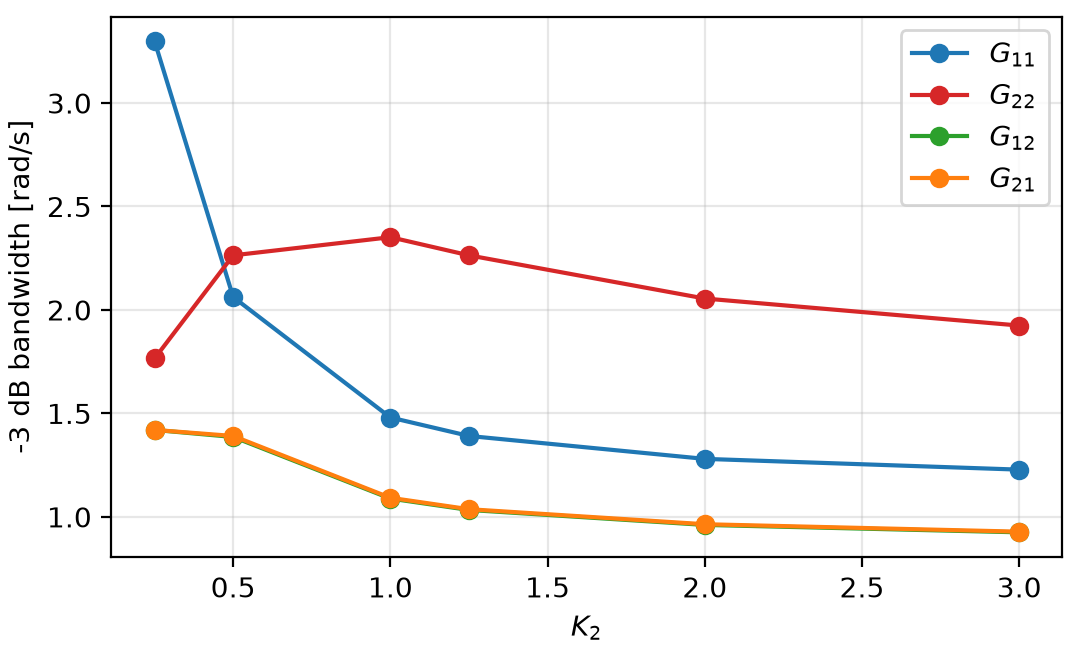
\includegraphics[width=0.4\textwidth]{en/fig_bw_vs_k2_a}}
\hfill
\subfloat[Resonance peak $M_r$]{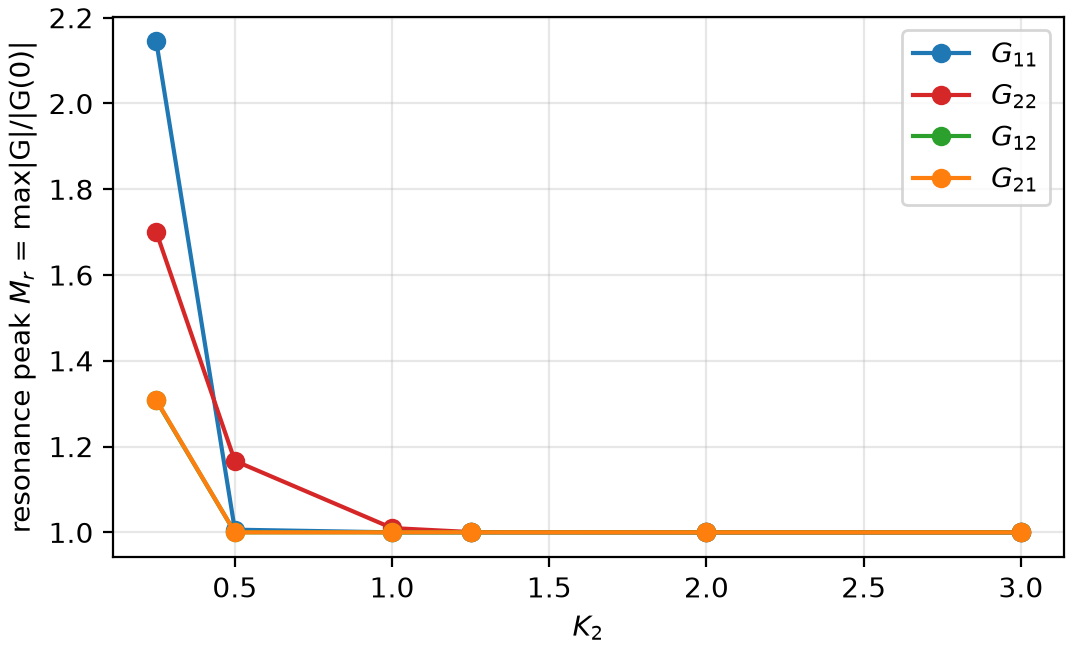
\includegraphics[width=0.4\textwidth]{en/fig_bw_vs_k2_b}}
\caption{Bandwidth and resonance peak as $K_2$ increases, with $K_1=1$.}\label{fig:bw}
\end{figure*}

\subsubsection{Bandwidth and resonance}
The bandwidth (BW) is the frequency up to which the channel follows a command well (where the magnitude drops 3 dB) and the resonance peak $M_r$ measures the maximum amplification with respect to low frequency ($M_r>1$ indicates a tendency to oscillate), as $K_2$ increases (Fig.~\ref{fig:bw}), with $K_2=0.25$ there is clear resonance ($M_r=2.15$ in $G_{11}$ and $1.70$ in $G_{22}$) and from $K_2\ge0.5$ all of them drop to $\approx1$, $K_2$ damps, the BW of $G_{22}$ (attitude) is best near $K_2\approx1$ (2.35 rad/s) and then drops a little, while that of $G_{11}$ (acceleration) drops from 3.3 to 1.2 rad/s as $K_2$ increases, a stronger nozzle rights the rocket sooner but also cuts the axial acceleration through gravity, it is a real compromise of the model, above about 2 rad/s the rocket does not follow commands, correcting faster only wastes nozzle.

\begin{figure}[!t]
\centering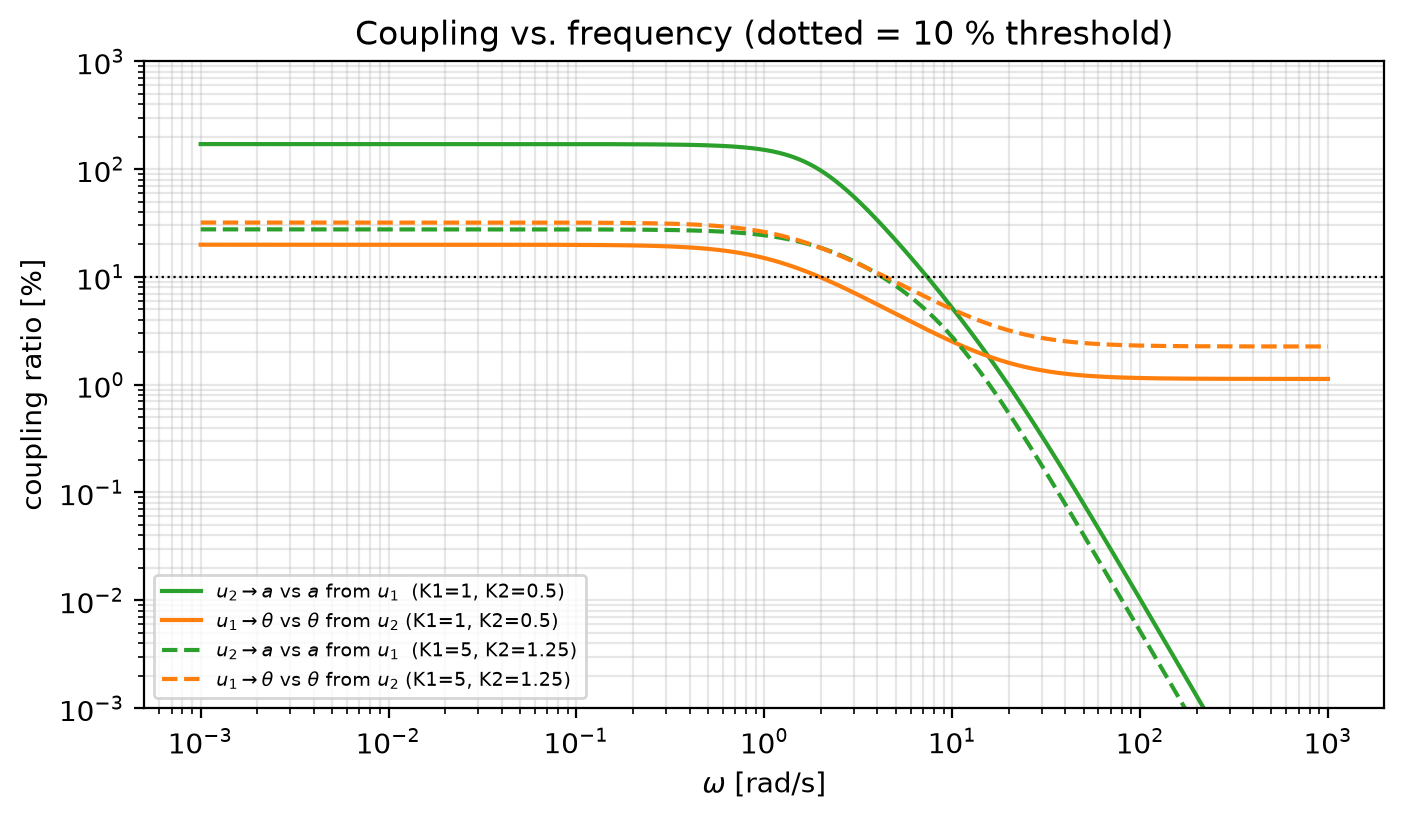
\includegraphics[width=\columnwidth]{fig_coupling_ratio.png}
\caption{Coupling (\%) against frequency, the dotted line is the 10\% threshold.}\label{fig:ratio}
\end{figure}

\subsubsection{When to treat them as independent}
Fig.~\ref{fig:ratio} compares $|G_{12}|$ against $|G_{11}|$ and $|G_{21}|$ against $|G_{22}|$ (with the same steps), the curves are flat at low frequency (the static coupling of $\sim170\%$ and 20\%) and fall as the frequency rises, with $(1,\,0.5)$, $u_2\to a$ exceeds 10\% up to 7.35 rad/s and $u_1\to\theta$ up to 1.96 rad/s, with $(5,\,1.25)$, $u_2\to a$ drops to 28\% but $u_1\to\theta$ rises to 32\% (the new gains spread the coupling more evenly) and both are below 10\% beyond about 4 rad/s, when the command varies fast (frequencies above about 5 rad/s) the two channels can be treated almost as independent, when it varies slowly, the rocket has to be considered as a single MIMO system.


\subsection{Observability and controllability}
\subsubsection{Observability}
The rocket has four states but only two are measured ($a$ and $\theta$), the others, $\omega$ and $\delta$, are not, can they be deduced from the sensors, if so, the system is \emph{observable}, it matters because the controller uses $\omega$ in Eq.~(\ref{eq:v2}), changing sensors does not change the rocket (same $A$, same poles), only the matrix $C$ changes, that is, what is seen, with only the accelerometer or with only the IMU,
\begin{align}
C_a&=\begin{bmatrix}1&0&0&0\end{bmatrix},\\
C_\theta&=\begin{bmatrix}0&1&0&0\end{bmatrix},
\end{align}
with both it is the nominal one, and if $\omega$ is also recorded to monitor structural loads, the row $[0\;0\;1\;0]$ is added.

Observability is verified with the rank of the matrix
\begin{equation}
O=\begin{bmatrix}C\\CA\\CA^2\\CA^3\end{bmatrix},
\end{equation}
where rank 4 means observable~\cite{nise}, in addition $\sigma_{\min}(O)$ is used, the smallest singular value, which says \emph{how well}, close to zero it is observable in theory but very sensitive to noise, with any sensor set the rank is 4, but the quality differs (Table~\ref{tab:obs}), with only $\theta$ the system is 45 times more fragile than with $a$, since the states have different units, $\sigma_{\min}$ is useful to compare sensors with each other, not as an absolute value.

\begin{table}[!t]
\centering\small
\caption{Observability according to the sensors.}\label{tab:obs}
\begin{tabular}{lcc}
\toprule
Sensors & Rank of $O$ & $\sigma_{\min}(O)$\\
\midrule
$a$ only & 4 & 0.993\\
$\theta$ only & 4 & 0.026\\
$a$ and $\theta$ & 4 & 1.172\\
$a$, $\theta$ and $\omega$ & 4 & 1.34\\
\bottomrule
\end{tabular}
\end{table}

The cause is the coupling itself, the accelerometer \emph{hears} the tilt through gravity ($-c_\theta\theta$ in $\dot a$), a strong path, while the IMU only sees the thrust through $k_\varepsilon=0.12$, a weak path, without coupling the rocket would be opaque, without gravity ($c_\theta=0$) with only the accelerometer the rank drops to 1 and without misalignment ($k_\varepsilon=0$) with only the IMU it drops to 3, in an unobservable system, an unstable mode could grow without the sensors seeing it and the computer would correct with a wrong state.

\begin{figure*}[!t]
\centering
\subfloat[$\omega$, observer with $a$ only]{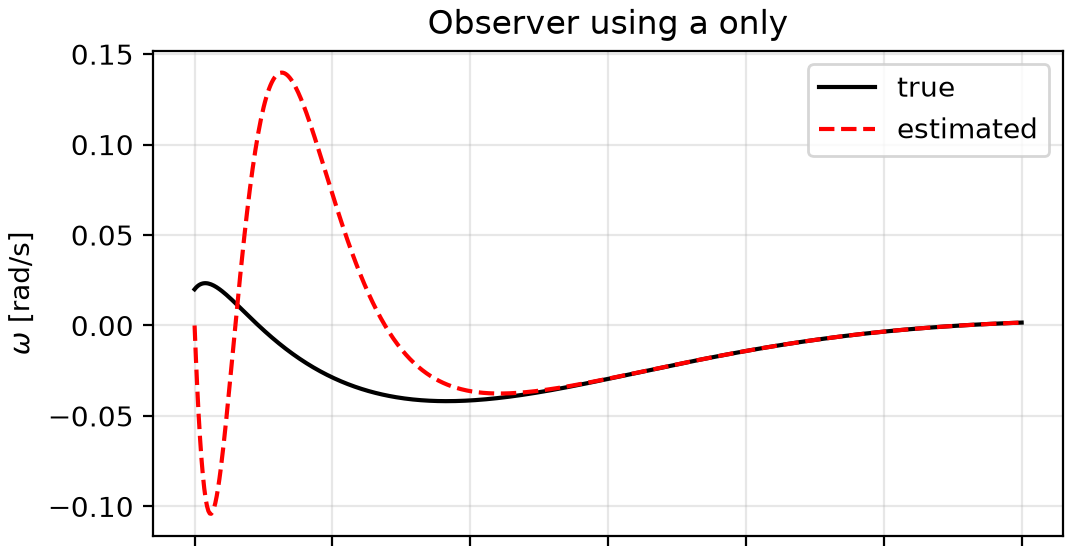
\includegraphics[width=0.4\textwidth]{en/fig_observer_a}}
\hfill
\subfloat[$\omega$, observer with $\theta$ only]{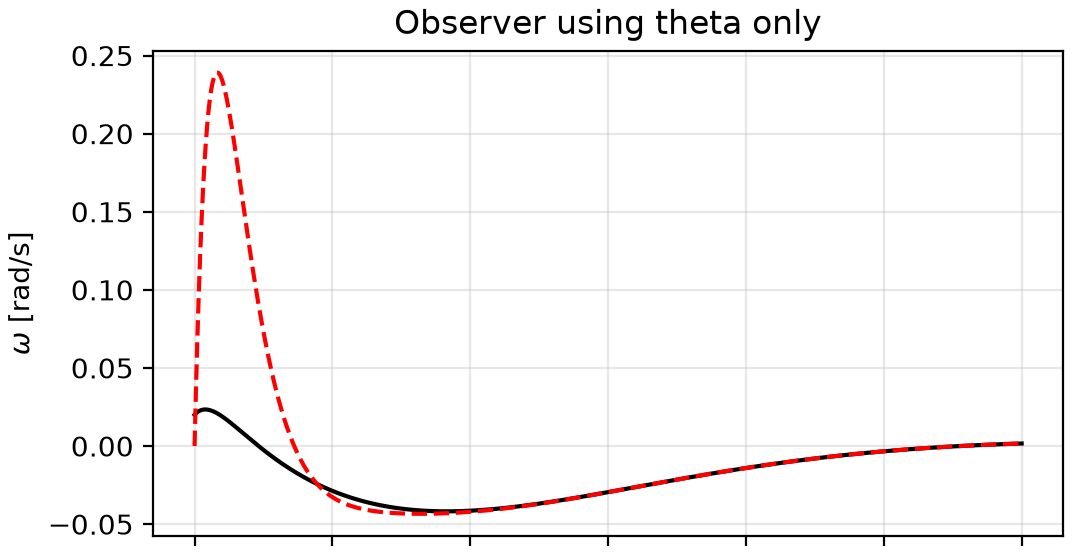
\includegraphics[width=0.4\textwidth]{en/fig_observer_b}}
\\
\subfloat[$\delta$, observer with $a$ only]{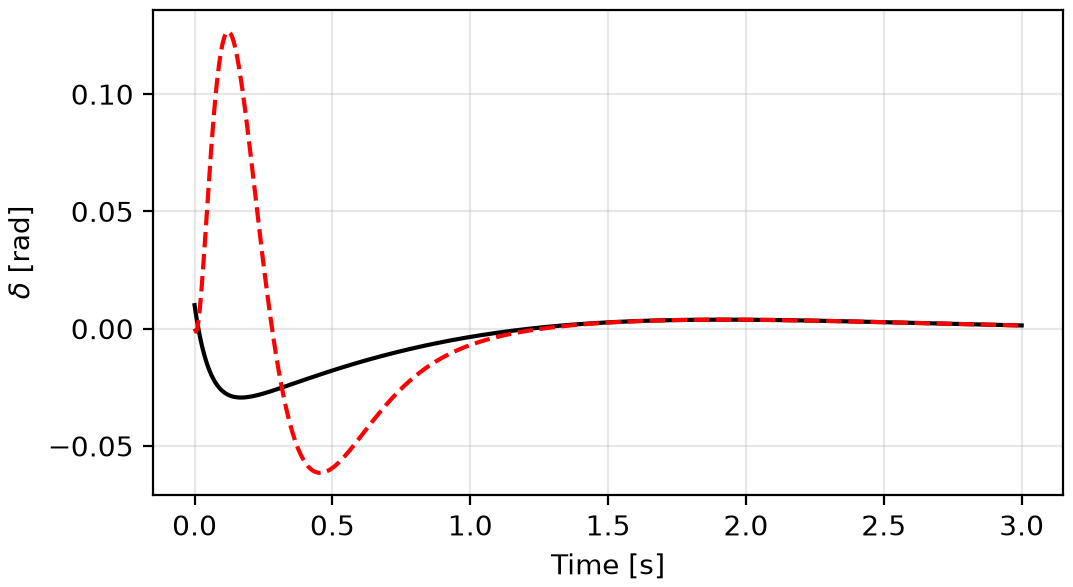
\includegraphics[width=0.4\textwidth]{en/fig_observer_c}}
\hfill
\subfloat[$\delta$, observer with $\theta$ only]{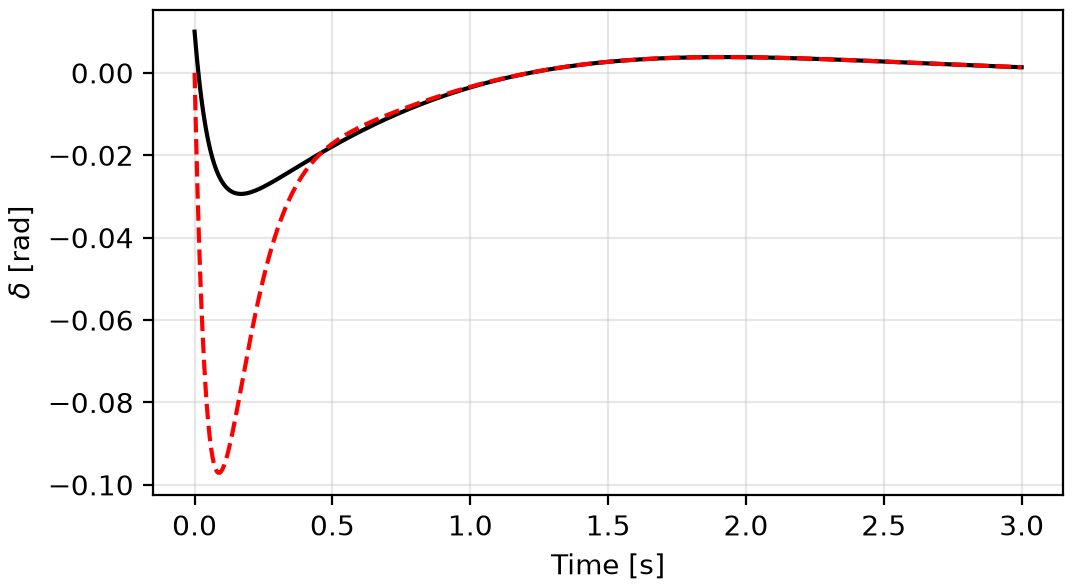
\includegraphics[width=0.4\textwidth]{en/fig_observer_d}}
\caption{Real states (black) and states estimated by the observer (red dashed).}\label{fig:obs}
\end{figure*}

To check that $\omega$ and $\delta$ can be reconstructed, a Luenberger observer was designed, a ``simulator of the rocket'' that is corrected with the measurements and that \emph{does not know} the initial state (it starts at zero), at first it is wrong and then it converges (Fig.~\ref{fig:obs}), with $a$ the curves overlap in 1 s and the error is $\sim10^{-9}$ at 3 s, with $\theta$ alone the initial peak is larger (the estimated $\omega$ reaches 0.24 rad/s when the real one is 0.02) and it demands an enormous correction gain ($|L|\approx3740$ against 22.5), the IMU is a narrow window onto $\omega$ and $\delta$, and reconstructing them amplifies the sensor noise.

\subsubsection{Controllability}
The inverse question is controllability, can the commands take the rocket to \emph{any} state, it was tested with both inputs, with $u_1$ alone (servo failure), with $u_2$ alone (thrust control failure), with the servo jammed ($\dot\delta=0$) and with $K_2=0$ (Table~\ref{tab:ctrb}), with $u_1$ alone the rank is 4, the rocket is controllable in theory, but with minimal authority ($\sigma_{\min}$ 907 times smaller), 10\% thrust tilts the rocket only $1.03^\circ$, with the servo jammed or with $K_2=0$ the rank drops to 3, the state $\delta$ is out of reach and the rocket is also unstable (pole $+0.557$), no control law can move an uncontrollable state, the nozzle is the critical piece and its loss is the worst scenario, the same as the instability with $K_2=0$, now seen as a lack of reach.

\begin{table}[!t]
\centering\small
\caption{Controllability in different scenarios.}\label{tab:ctrb}
\begin{tabular}{lccc}
\toprule
Scenario & Rank & $\sigma_{\min}$ & Stable\\
\midrule
$u_1$ and $u_2$ (nominal) & 4 & 1.3 & yes\\
$u_1$ only & 4 & 0.0014 & yes\\
$u_2$ only & 4 & 1.3 & yes\\
jammed servo ($u_1$ only) & 3 & 0 & no\\
$K_2=0$ & 3 & 0 & no\\
\bottomrule
\end{tabular}
\end{table}


\subsection{Gain selection and sampling period}
\subsubsection{Selection criteria}
So far almost every pair $(K_1,K_2)$ with $K_2\gtrsim0.09$ is stable, but that is not enough, the nominal one overshoots 16.4\% and takes 3.6 s, gains have to be chosen that give good performance without wasting too much nozzle or coupling too much, a grid of 2400 pairs was swept ($K_1\in[0.5,\,20]$, $K_2\in[0.05,\,3]$) with five criteria on the response to the steps of $10\%$ and $5^\circ$ (the same as in the coupling analysis), overshoot $M_p\le10\%$, settling time $t_s\le3$ s, final error $\le5\%$, maximum nozzle deflection $\le5^\circ$ and $G_{11}(0)>0$, among the points that meet everything, the one with the least coupling is preferred, measured as the worse of the two percentages, the limits are a design choice of the team, the nozzle limit also refers to those steps.

\begin{figure*}[!t]
\centering
\subfloat[Overshoot]{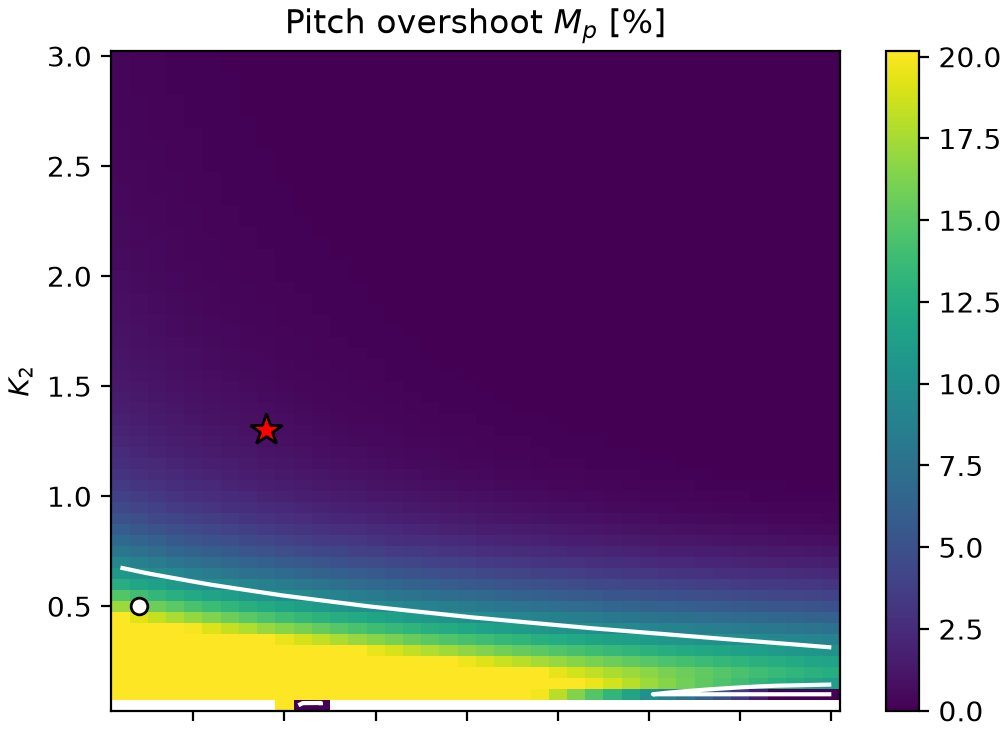
\includegraphics[width=0.32\textwidth]{en/fig_metric_maps_a}}
\hfill
\subfloat[Settling time]{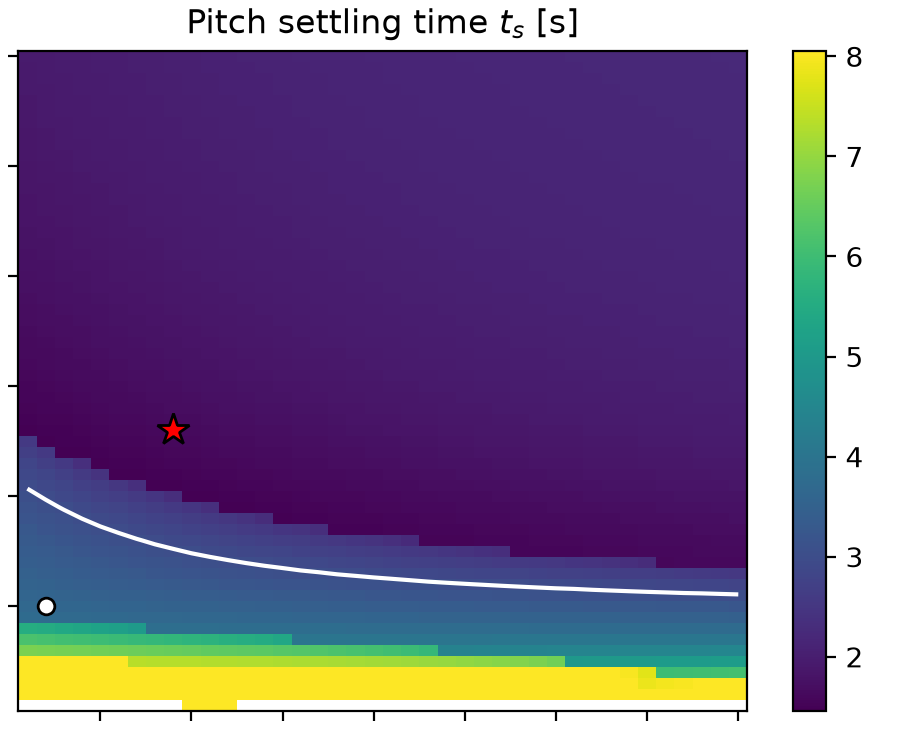
\includegraphics[width=0.32\textwidth]{en/fig_metric_maps_b}}
\hfill
\subfloat[Final error]{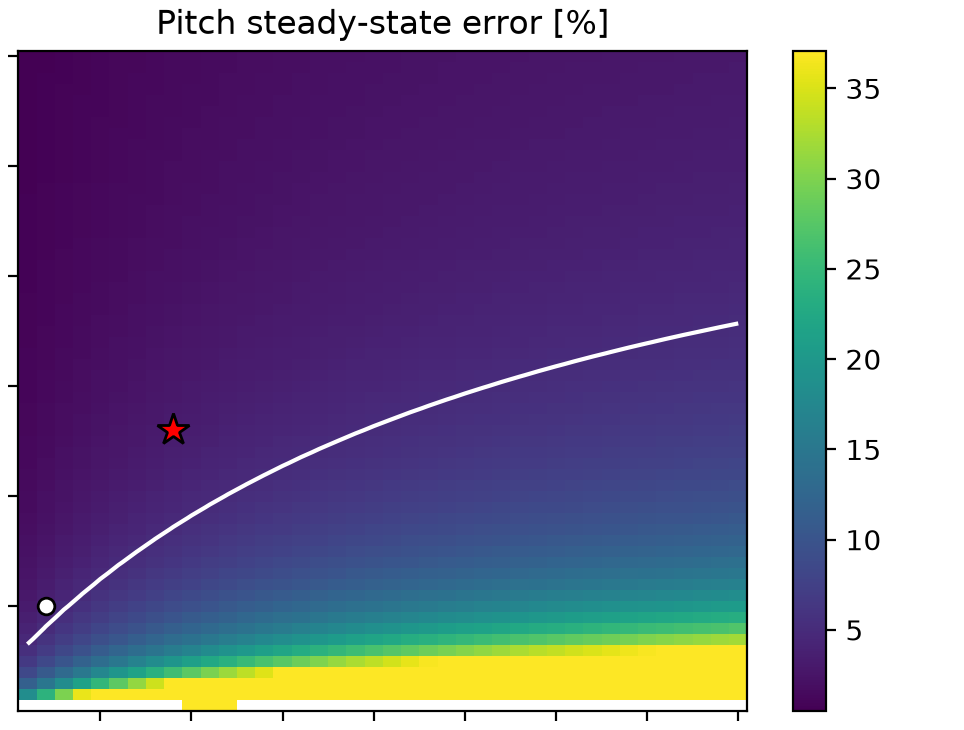
\includegraphics[width=0.32\textwidth]{en/fig_metric_maps_c}}
\\
\subfloat[Nozzle deflection]{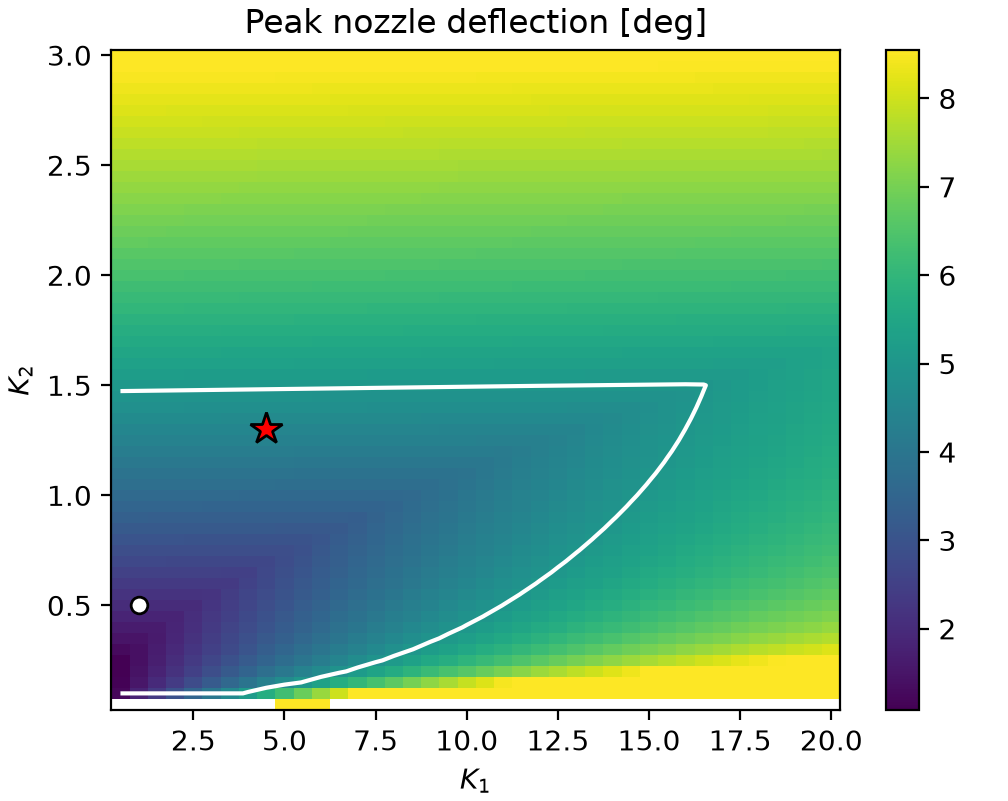
\includegraphics[width=0.32\textwidth]{en/fig_metric_maps_d}}
\hfill
\subfloat[Worst coupling]{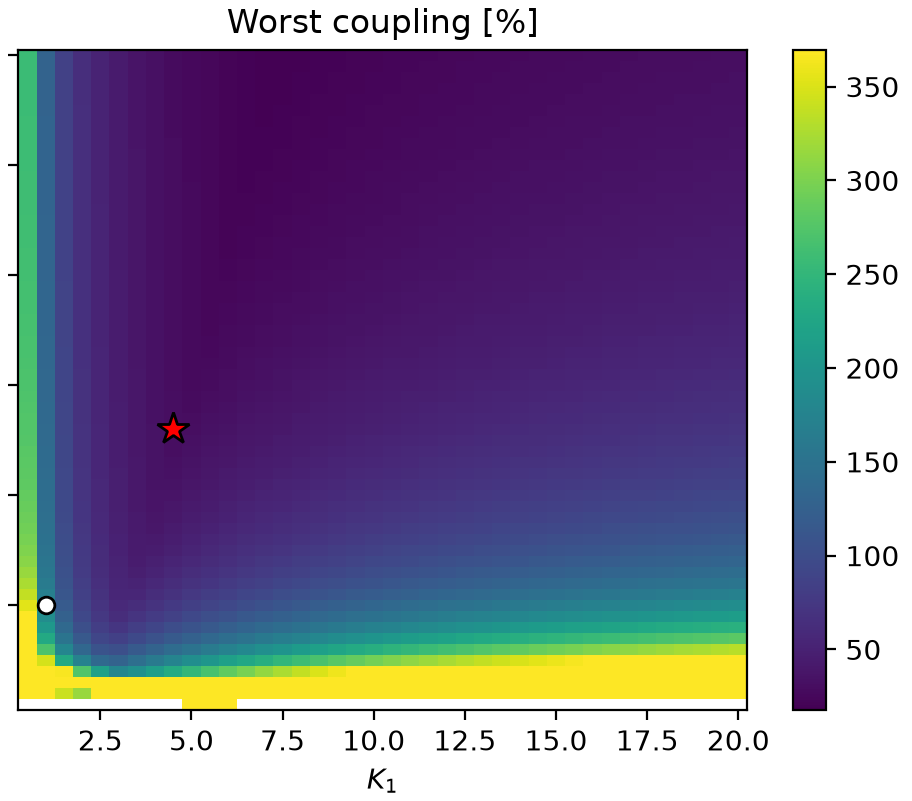
\includegraphics[width=0.32\textwidth]{en/fig_metric_maps_e}}
\hfill
\subfloat[Feasible and recommended zones]{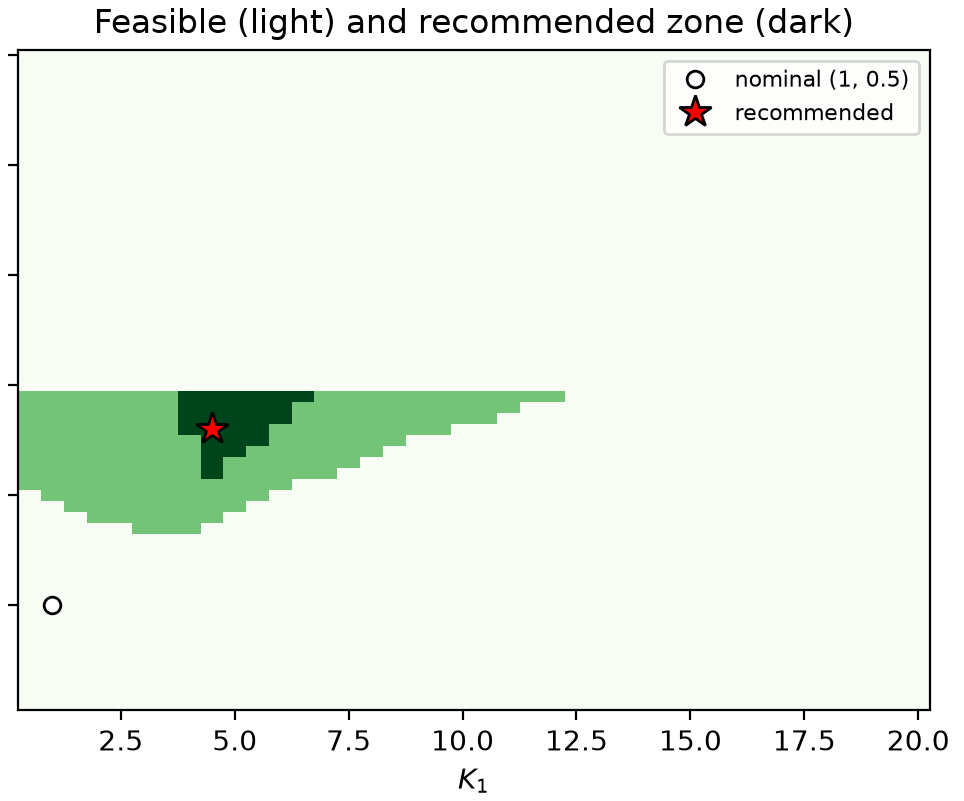
\includegraphics[width=0.32\textwidth]{en/fig_metric_maps_f}}
\caption{One map per criterion over the $(K_1,K_2)$ plane, the white line is the limit, $\circ$ is the nominal and $\star$ the recommended point, in (f) the feasible zone is light and the recommended one is dark.}\label{fig:maps}
\end{figure*}

\subsubsection{Feasible and recommended gains}
Fig.~\ref{fig:maps} is read as follows, the color is the value of the criterion, dark is low and yellow is high, and since the five are ``costs'', dark is good, the scale is cut at the 95th percentile so that the few almost-unstable points do not crush the colors, the white line is the limit and the dark side meets it.
\begin{itemize}
  \item \emph{Overshoot and time} improve as $K_2$ rises (panels (a) and (b), dark), with a small $K_2$ the nozzle barely counteracts $\mu$, the oscillatory poles are poorly damped and the rocket pitches too much, the nominal is below the line (16.4\% and 3.64 s).
  \item \emph{Final error}, the line rises with $K_1$, from $K_2\approx0.35$ to $\approx1.8$ for $K_1=20$, because more thrust tilts the rocket too much through $k_\varepsilon$ ($G_{22}(0)=1.04$ with $K_1=1$ and $1.14$ with $K_1=10$) and more $K_2$ is needed for the nozzle to hold the requested angle.
  \item \emph{Nozzle deflection}, it is the only criterion that encloses a region (only 683 of 2400 points meet it), above ($K_2\gtrsim1.5$) the nozzle commands too much for each degree of error, to the right the larger thrust forces it to work harder, it sets the \emph{ceiling} $K_2\approx1.45$.
  \item \emph{Coupling}, it has no limit, it is what is minimized, it is minimal toward $K_1\gtrsim5$ with medium or high $K_2$.
\end{itemize}
The feasible zone (187 points, $K_1\in[0.5,\,12]$, $K_2\in[0.85,\,1.45]$) is the intersection, the flat ceiling is the nozzle and the diagonal lower edge is the final error, which cuts the ceiling near $K_1\approx12$, the recommended zone, with coupling within 25\% of the best feasible one, is
\begin{gather}
K_1\in[4,\,6.5],\qquad K_2\in[1.1,\,1.45],\nonumber\\
(K_1,K_2)_{\text{rec}}=(4.5,\ 1.3).
\end{gather}
Table~\ref{tab:rec} compares the nominal with the recommended point, the overshoot drops almost to zero and the time to less than half, and the coupling is spread (177\% to 31\% in $u_2\to a$) at the cost of raising the other from 21\% to 28\%, the nozzle works harder ($4.5^\circ$ of the $5^\circ$ allowed), the poles also change, the slow mode moves to $-1.6$ and a fast oscillatory pair $-9.2\pm4.3j$ appears (the servo now mixes with the rotation), it is a compromise, not a unique optimum.

\begin{table}[!t]
\centering\small
\caption{Nominal against recommended.}\label{tab:rec}
\begin{tabular}{p{2.3cm}p{2.6cm}p{2.6cm}}
\toprule
 & Nominal $(1,\,0.5)$ & Recommended $(4.5,\,1.3)$\\
\midrule
Overshoot $M_p$ of $\theta$ & 16.4\% & 0.82\%\\
Settling time & 3.64 s & 1.62 s\\
Final error & 4.03\% & 3.25\%\\
Maximum nozzle deflection & $2.0^\circ$ & $4.5^\circ$\\
Coupling $u_2\to a$ / $u_1\to\theta$ & 177\% / 21\% & 31\% / 28\%\\
Poles [s$^{-1}$] & $-17.3$, $-2.1$, $-1.07\pm1.2j$ & $-9.2\pm4.3j$, $-1.6\pm0.46j$\\
\bottomrule
\end{tabular}
\end{table}

\subsubsection{Sampling period}
In reality the controller is a computer, it measures, computes and commands every $T$ seconds and keeps the command constant between samples (zero-order hold, the command is a staircase), if $T$ is too large, the rocket changed too much between corrections and the loop becomes unstable, like correcting a steering wheel once per second, in addition the computation takes time, which is modeled with a one-sample delay, the question is how large $T$ can be and whether $T=0.05$ s is sufficient.

\begin{figure*}[!t]
\centering
\subfloat[Instantaneous computer]{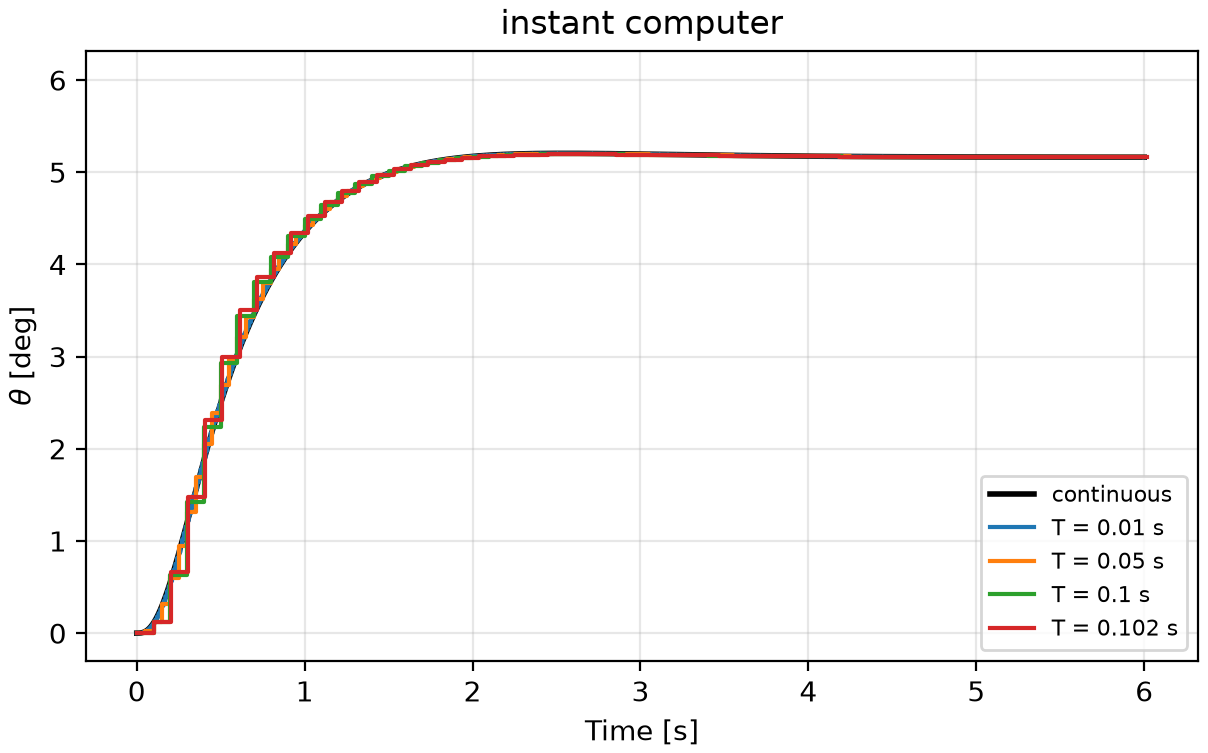
\includegraphics[width=0.42\textwidth]{en/fig_sampling_a}}
\hfill
\subfloat[One-sample computation delay]{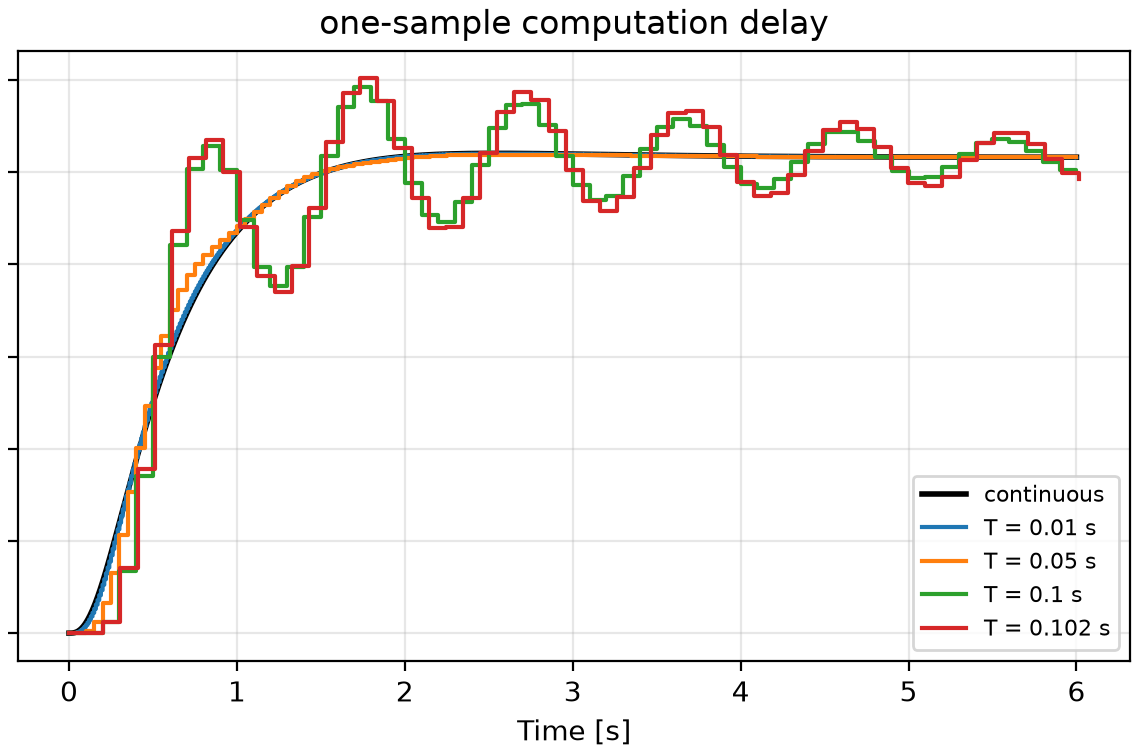
\includegraphics[width=0.42\textwidth]{en/fig_sampling_b}}
\caption{Response of $\theta$ to $u_2=5^\circ$ with the recommended gains, continuous loop (black) against sampled (steps).}\label{fig:sampling}
\end{figure*}

In Fig.~\ref{fig:sampling}, with an instantaneous computer, even $T=0.1$ s almost coincides with the continuous response, with delay, $T=0.05$ s still works well, but with $T=0.1$ s the response oscillates around $5^\circ$ ($\pm1^\circ$) and does not finish settling, it is about to become unstable, a delay makes the correction arrive late, and in a rocket with a fast oscillatory mode such as $-9.2\pm4.3j$ that is dangerous, the rule of thumb asks for between 10 and 20 samples within the rise time, with $T=0.05$ s there are 19 (rise time of 0.97 s).

\begin{figure}[!t]
\centering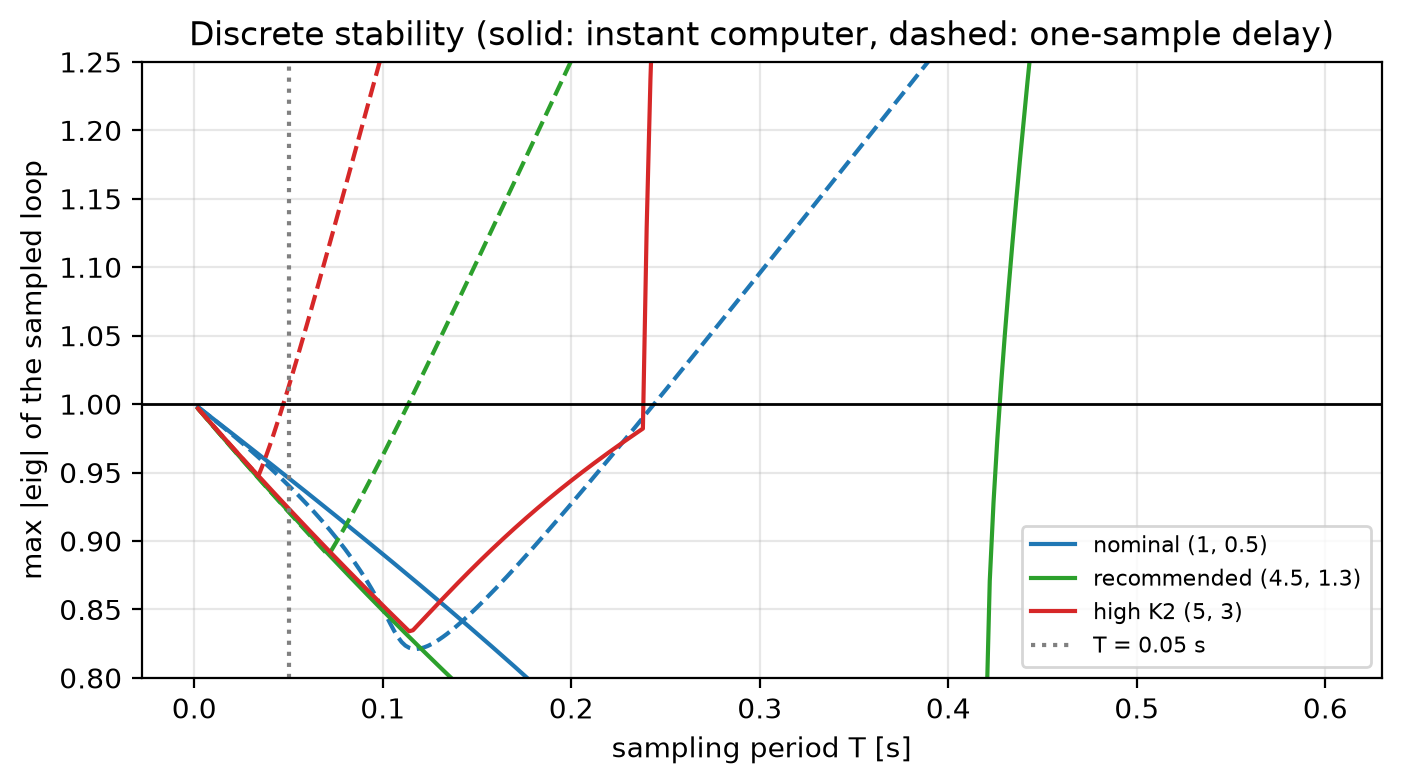
\includegraphics[width=\columnwidth]{fig_sampling_stability.png}
\caption{Spectral radius against $T$ (solid, without delay, dashed, with a one-sample delay).}\label{fig:rho}
\end{figure}

The spectral radius summarizes discrete stability in a single number, as long as it is below 1 the loop is stable (Fig.~\ref{fig:rho}), each curve drops to a minimum and then rises until it crosses 1, and that crossing is $T_{\max}$, Table~\ref{tab:tmax} shows that with the recommended gains $T_{\max}$ in the worst case (with delay) is 0.114 s, that is, $2.3$ times the chosen period ($0.114/0.05$), the computer could be 2.3 times slower before the loop becomes unstable, it is a safety margin, not an improvement of the response, and it is smaller than that of the nominal ($4.9\times$), raising $K_2$ improves the overshoot and the settling time, but it spends sampling margin, with a high $K_2$, such as $(5,\,3)$, the ratio is less than one and the loop would be unstable with $T=0.05$ s.

\begin{table}[!t]
\centering\small\setlength{\tabcolsep}{3pt}
\caption{$T_{\max}$ and margin ($=T_{\max}$ with delay$/0.05$ s).}\label{tab:tmax}
\begin{tabular}{lrrr}
\toprule
Gains & Without delay & With delay & Margin\\
\midrule
Nominal $(1,\,0.5)$ & 0.999 s & 0.244 s & $4.9\times$\\
Recommended $(4.5,\,1.3)$ & 0.427 s & 0.114 s & $2.3\times$\\
High $K_2$ $(5,\,3)$ & 0.239 s & 0.047 s & $0.9\times$\\
\bottomrule
\end{tabular}
\end{table}

\begin{figure}[!t]
\centering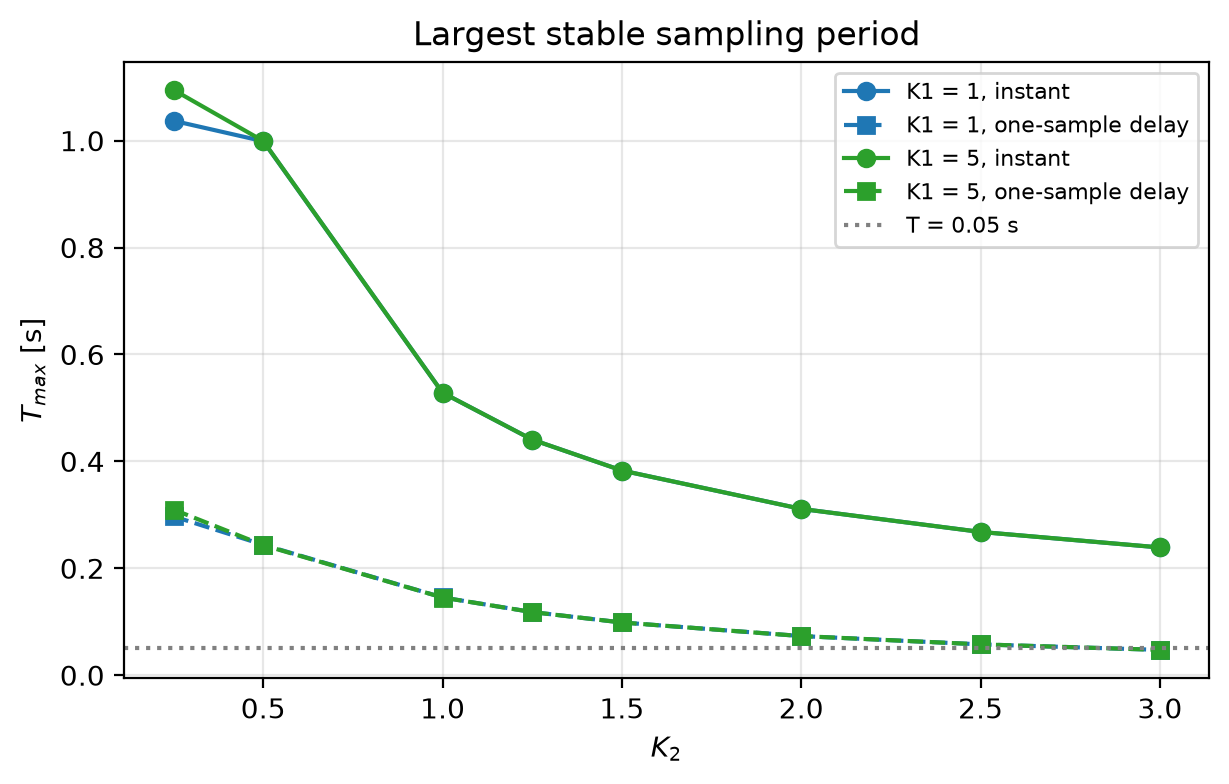
\includegraphics[width=\columnwidth]{fig_tmax_vs_k2.png}
\caption{$T_{\max}$ against $K_2$ for $K_1=1$ and $K_1=5$.}\label{fig:tmaxk2}
\end{figure}

Fig.~\ref{fig:tmaxk2} shows that $K_1$ barely affects $T_{\max}$ (the curves coincide), what lowers it is $K_2$, from $\sim1$ s to $\sim0.24$ s without delay and from $\sim0.3$ to $\sim0.05$ s with delay, $K_2$ governs the servo, the fast element (pole $-17$), a servo with more gain is more ``nervous'' and needs to be corrected more often, so raising $K_2$ as much as possible is not enough, the nozzle ceiling is one limit, and this is another, a sampling one, the bandwidth of the rocket ($\sim2$ rad/s) is far below the sampling frequency ($2\pi/0.05\approx126$ rad/s), so sampling is not the limitation, the computation delay combined with high values of $K_2$ is.


\subsection{Model variations, variable mass and yaw}
\subsubsection{Variable mass}
The engine burns fuel, with constant thrust,
\begin{equation}
\dot m=-\frac{F_T}{I_{sp}g_0},
\end{equation}
and the inertia is assumed proportional to the mass, with
\begin{equation}
\rho(t)=\frac{m_0}{m(t)}\ge1
\end{equation}
($\rho=2$ is a rocket at half of its mass), the coefficients that contain $1/m$ or $1/I$ grow with $\rho$, $k_a$, $k_\delta$, $\mu$ and $k_\varepsilon$ are proportional to $\rho$, while $c_\theta$ and the constants of the engine and of the servo do not change, with variable inertia the moment balance is
\begin{equation}
I\dot\omega+\dot I\omega=M,
\end{equation}
which adds a term that does not exist in the constant-coefficient model,
\begin{equation}
\dot\omega=\frac{M}{I}-\frac{\dot I}{I}\,\omega,
\end{equation}
since
\begin{equation}
\frac{\dot I}{I}=-\frac{\dot\rho}{\rho},
\end{equation}
the damping becomes
\begin{equation}
a_{d,\mathrm{eff}}=\rho\,a_{d0}-\frac{\dot\rho}{\rho}
\end{equation}
(a small anti-damping), the model is that of Eqs.~(\ref{eq:a})--(\ref{eq:de}) with time-dependent coefficients,
\begin{equation}
\dot x=A(t)x+B(t)u,
\end{equation}
where only $A_{11}$, $A_{31}$, $A_{32}$, $A_{33}$, $A_{34}$ and $B_{11}$ change, the gains $g_1$, $g_3$, $g_4$, $g_5$, $g_6$ and $g_7$ of the diagram (Fig.~\ref{fig:timevar}).

\begin{figure}[!t]
\centering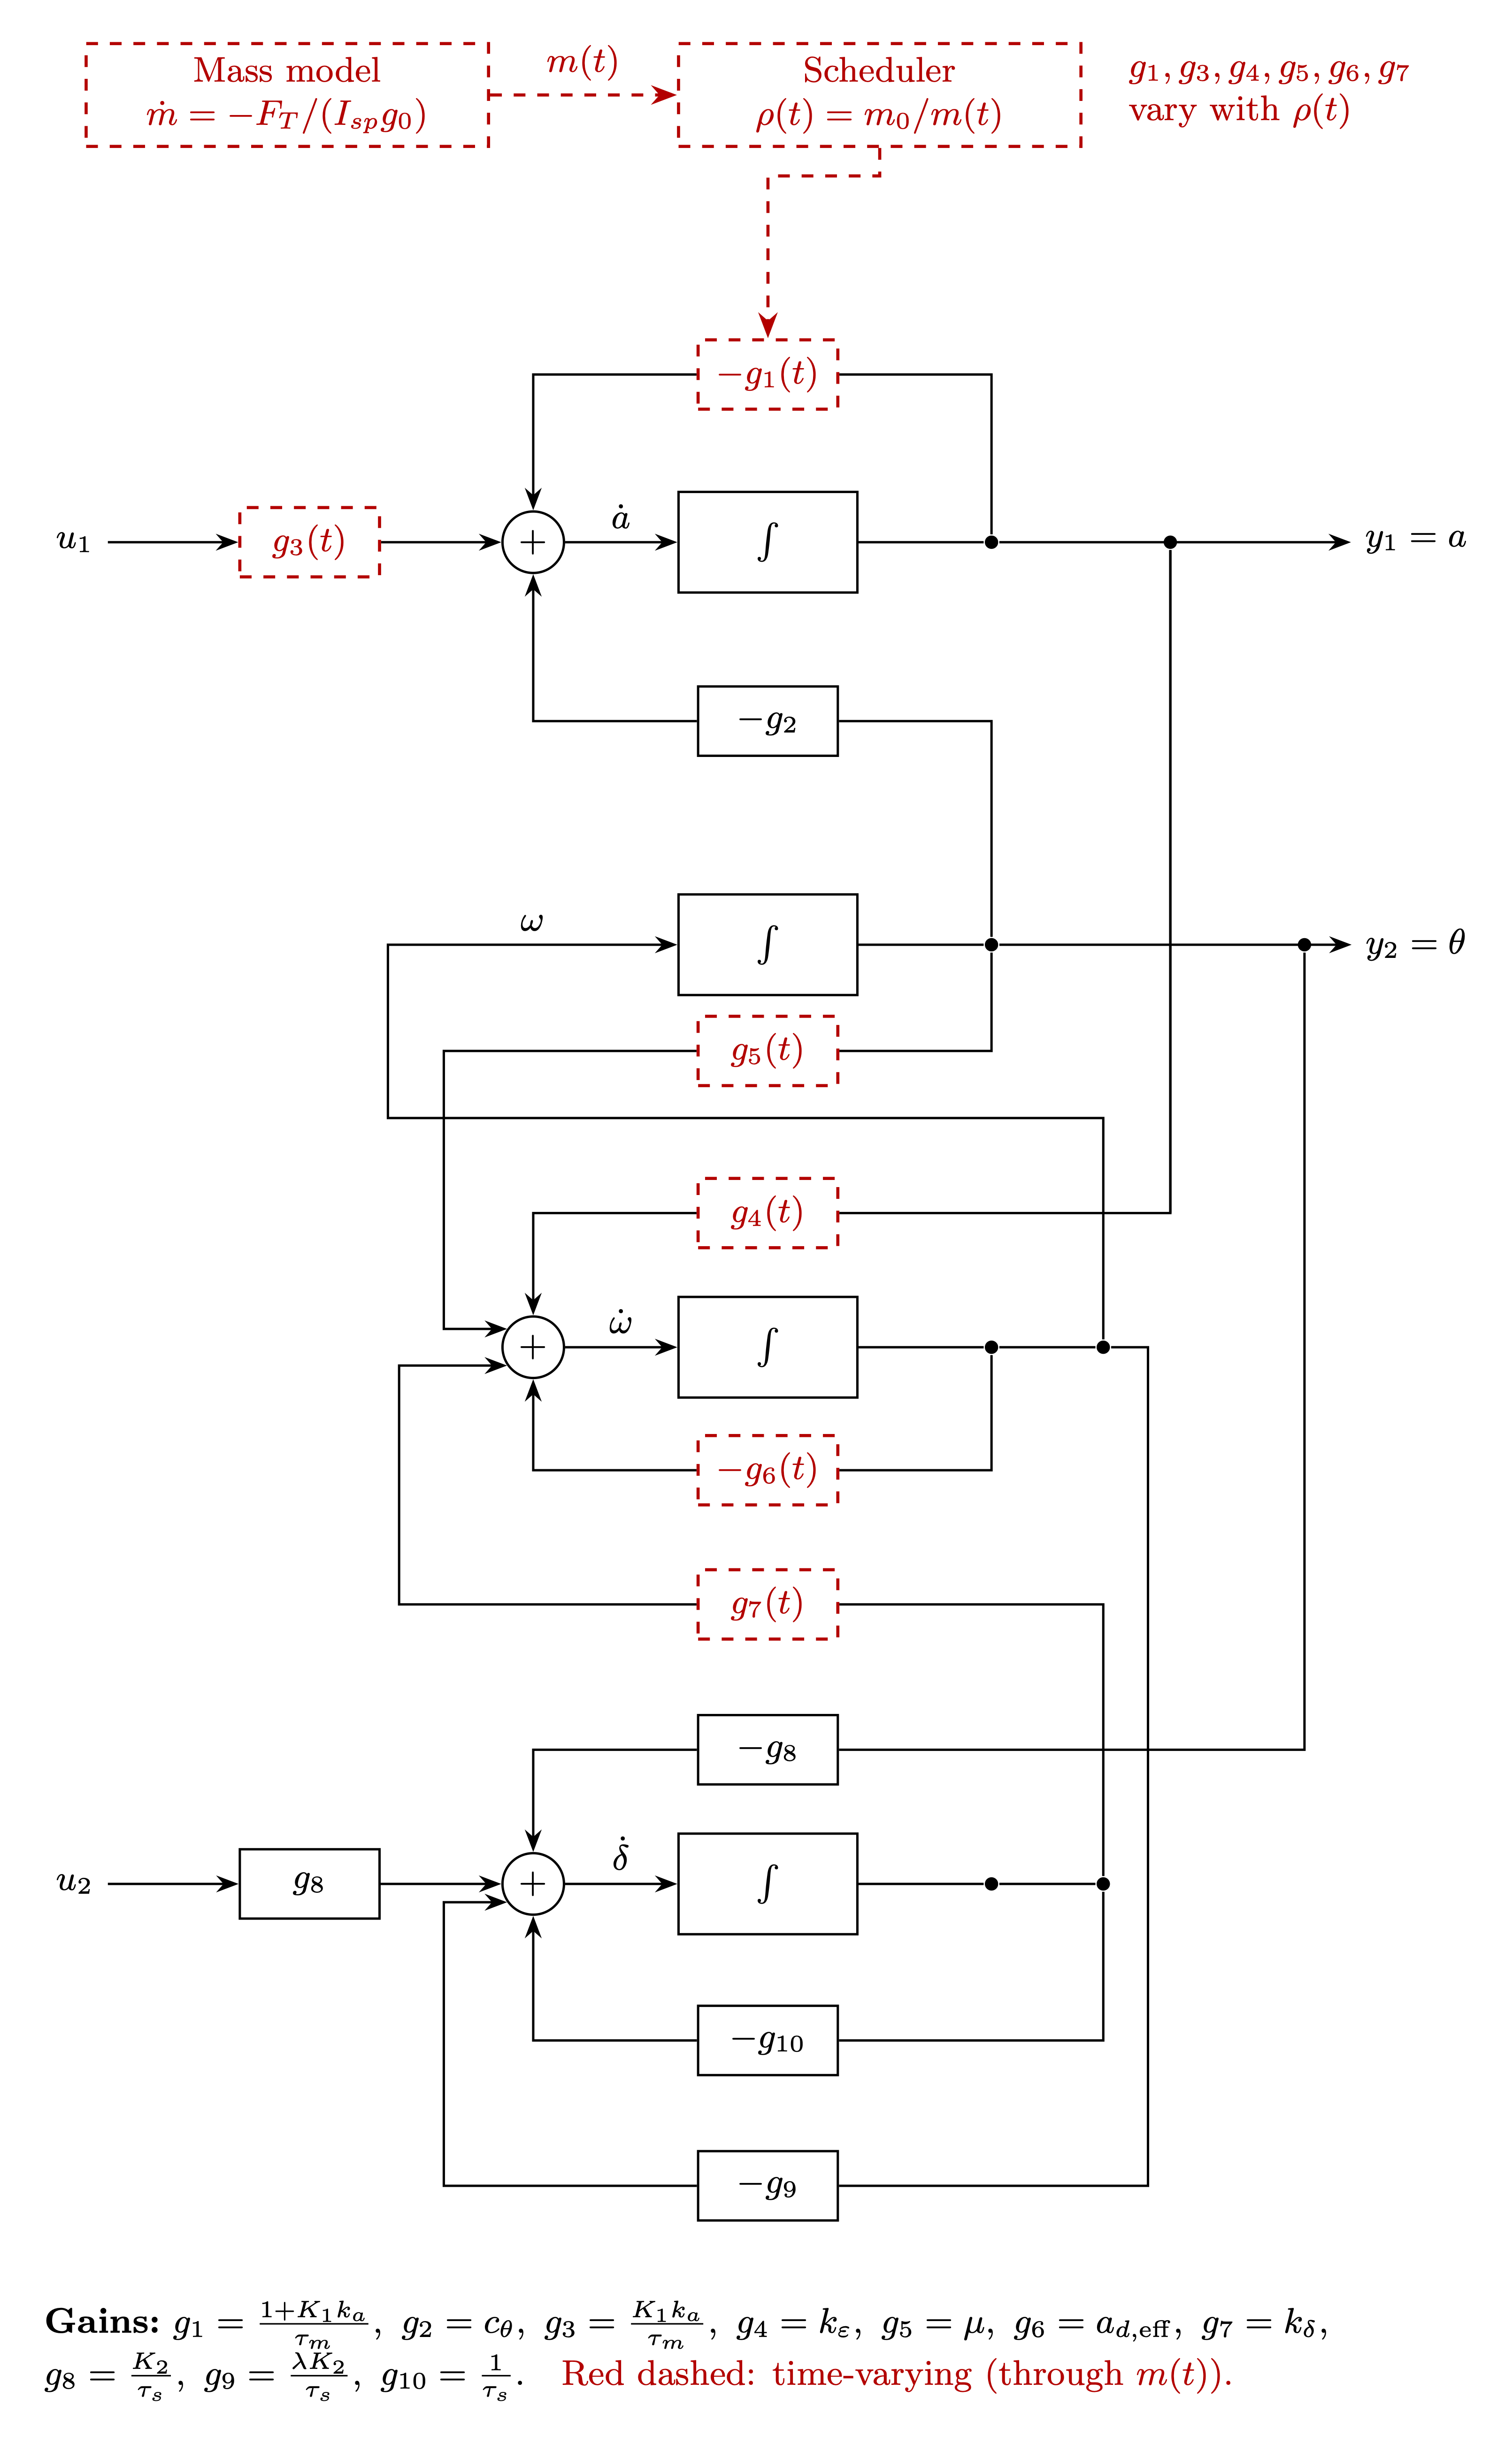
\includegraphics[width=\columnwidth]{fig_f15_timevar.png}
\caption{Diagram with variable mass, in red, the gains that change with $m(t)$ through $\rho(t)$.}\label{fig:timevar}
\end{figure}

With changing coefficients $G(p)$ and fixed poles no longer exist, because both assume constant coefficients, the state-transition matrix $\Phi(t,t_0)$ is used instead, freezing $\rho$ at each instant gives an approximate check, valid while the mass changes slowly compared with the speed of the loop ($\sim1$ s), but it does not prove stability, since the loop gain grows with $\rho$, it is convenient to \emph{schedule the gains},
\begin{equation}
K_1(t)=\frac{K_1}{\rho},\qquad K_2(t)=\frac{K_2}{\rho},
\end{equation}
which keep $K_1k_a(t)$ and $k_\delta(t)K_2(t)$ constant, in Fig.~\ref{fig:frozen}, with fixed gains the slow poles barely move ($\approx-1.6$), but the fast pair moves away from the real axis, with an imaginary part from $\pm4.3$ ($\rho=1$) to $\pm12.4$ ($\rho=2$), the rocket becomes more ``vibrating'' because the same gain is now stronger relative to the mass, it remains stable, but $T_{\max}$ with delay drops from 0.114 s to 0.058 s with $\rho=2$, almost equal to the chosen period of 0.05 s, with scheduled gains the poles barely move and $T_{\max}$ stays between 0.114 and 0.123 s, the recommended gains are valid at the start of the flight and it is convenient to readjust them with the mass to keep the sampling margin.

\begin{figure*}[!t]
\centering
\subfloat[Fixed gains]{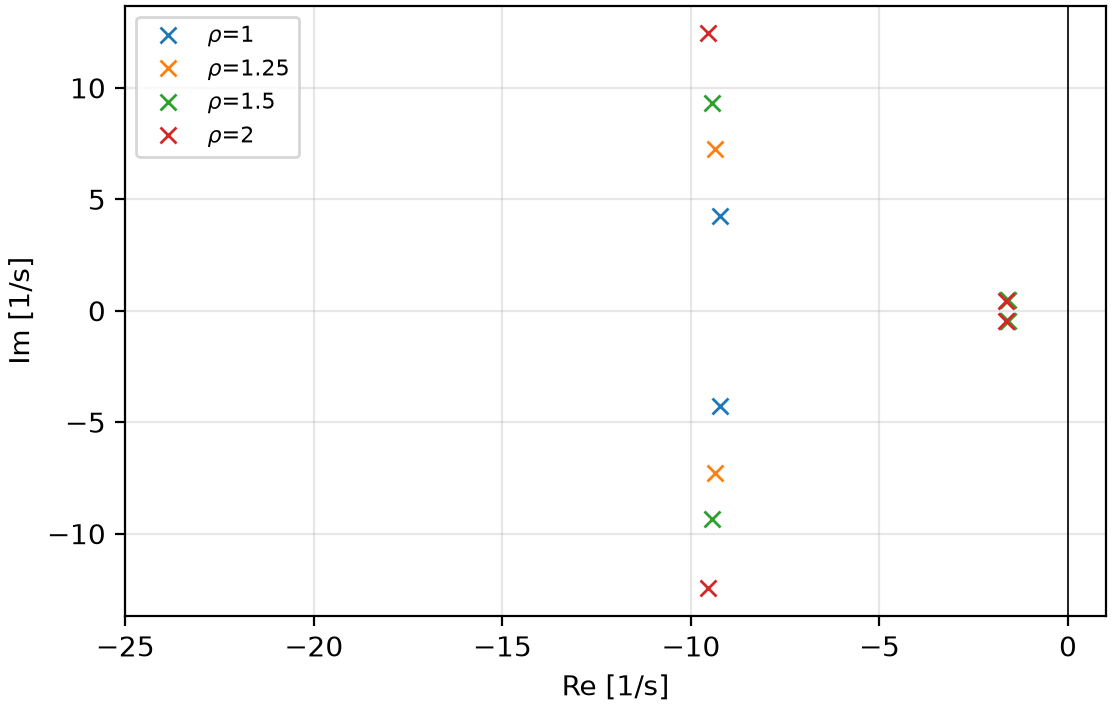
\includegraphics[width=0.4\textwidth]{en/fig_f15_frozen_poles_a}}
\hfill
\subfloat[Gains scheduled with $1/\rho$]{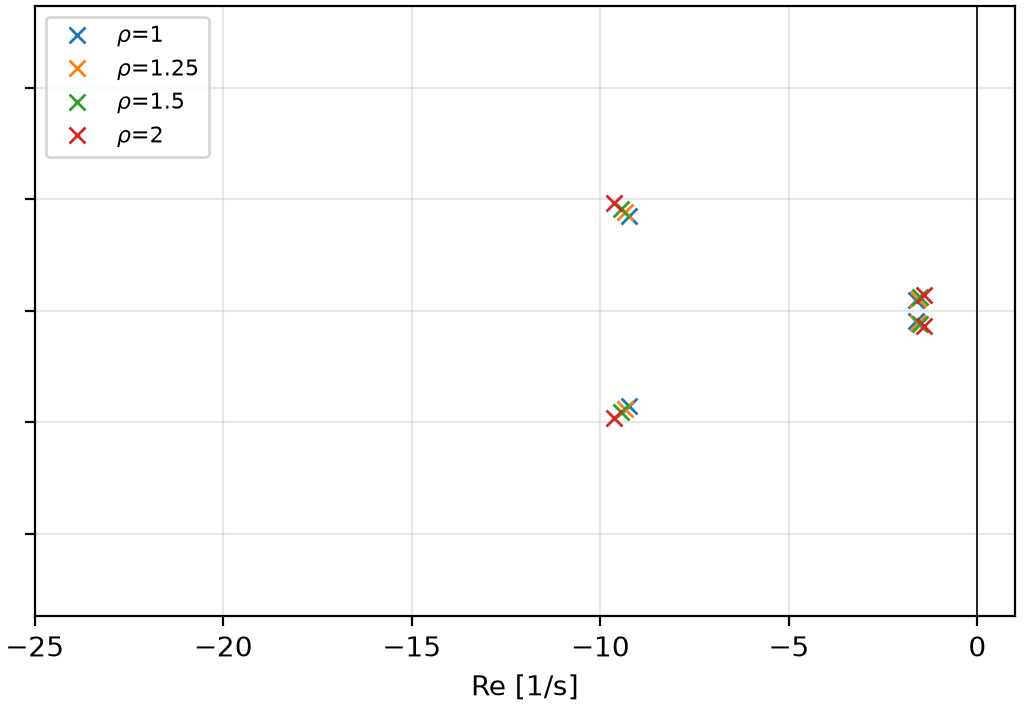
\includegraphics[width=0.4\textwidth]{en/fig_f15_frozen_poles_b}}
\caption{Frozen-time poles as the mass varies.}\label{fig:frozen}
\end{figure*}

\subsubsection{Yaw as a third channel}
A rocket is almost symmetric around its axis, so yaw (lateral rotation) repeats the pitch in the perpendicular plane, with its own nozzle, the yaw angle $\psi$, its rate $r=\dot\psi$ and the lateral deflection $\zeta$ are added, with a command $u_3$ and a gain $K_3$ (small angles and no roll),
\begin{align}
\dot\psi&=r,\\
\dot r&=k_{\varepsilon\psi}\,a+\mu_\psi\,\psi-a_{d\psi}\,r+k_{\delta\psi}\,\zeta,\label{eq:yaw1}\\
\dot\zeta&=-\tfrac{1}{\tau_s}\,\zeta-\tfrac{K_3}{\tau_s}\,\psi-\tfrac{\lambda K_3}{\tau_s}\,r+\tfrac{K_3}{\tau_s}\,u_3,\label{eq:yaw2}
\end{align}
with $\mu_\psi=\mu$, $a_{d\psi}=a_d$, $k_{\delta\psi}=k_\delta$ and $k_{\varepsilon\psi}=k_\varepsilon$ (symmetric rocket), the state, the input and the output are
\begin{align}
x&=[a,\theta,\omega,\delta,\psi,r,\zeta]^T,\\
u&=[u_1,u_2,u_3]^T,\\
y&=[a,\theta,\psi]^T,
\end{align}
that is, 7 states, 3 inputs and 3 outputs, with $A$ block triangular,
\begin{equation}
A=\begin{bmatrix}A_{\text{pitch}}&0\\K_{\psi a}&A_{\text{yaw}}\end{bmatrix},\qquad B_{\text{yaw}}=\begin{bmatrix}0\\0\\K_3/\tau_s\end{bmatrix},
\end{equation}
where $K_{\psi a}$ has a single nonzero entry, $k_{\varepsilon\psi}$ (from $a$ to $\dot r$), and it is the only link between the two planes (Fig.~\ref{fig:yaw}).

\begin{figure}[!t]
\centering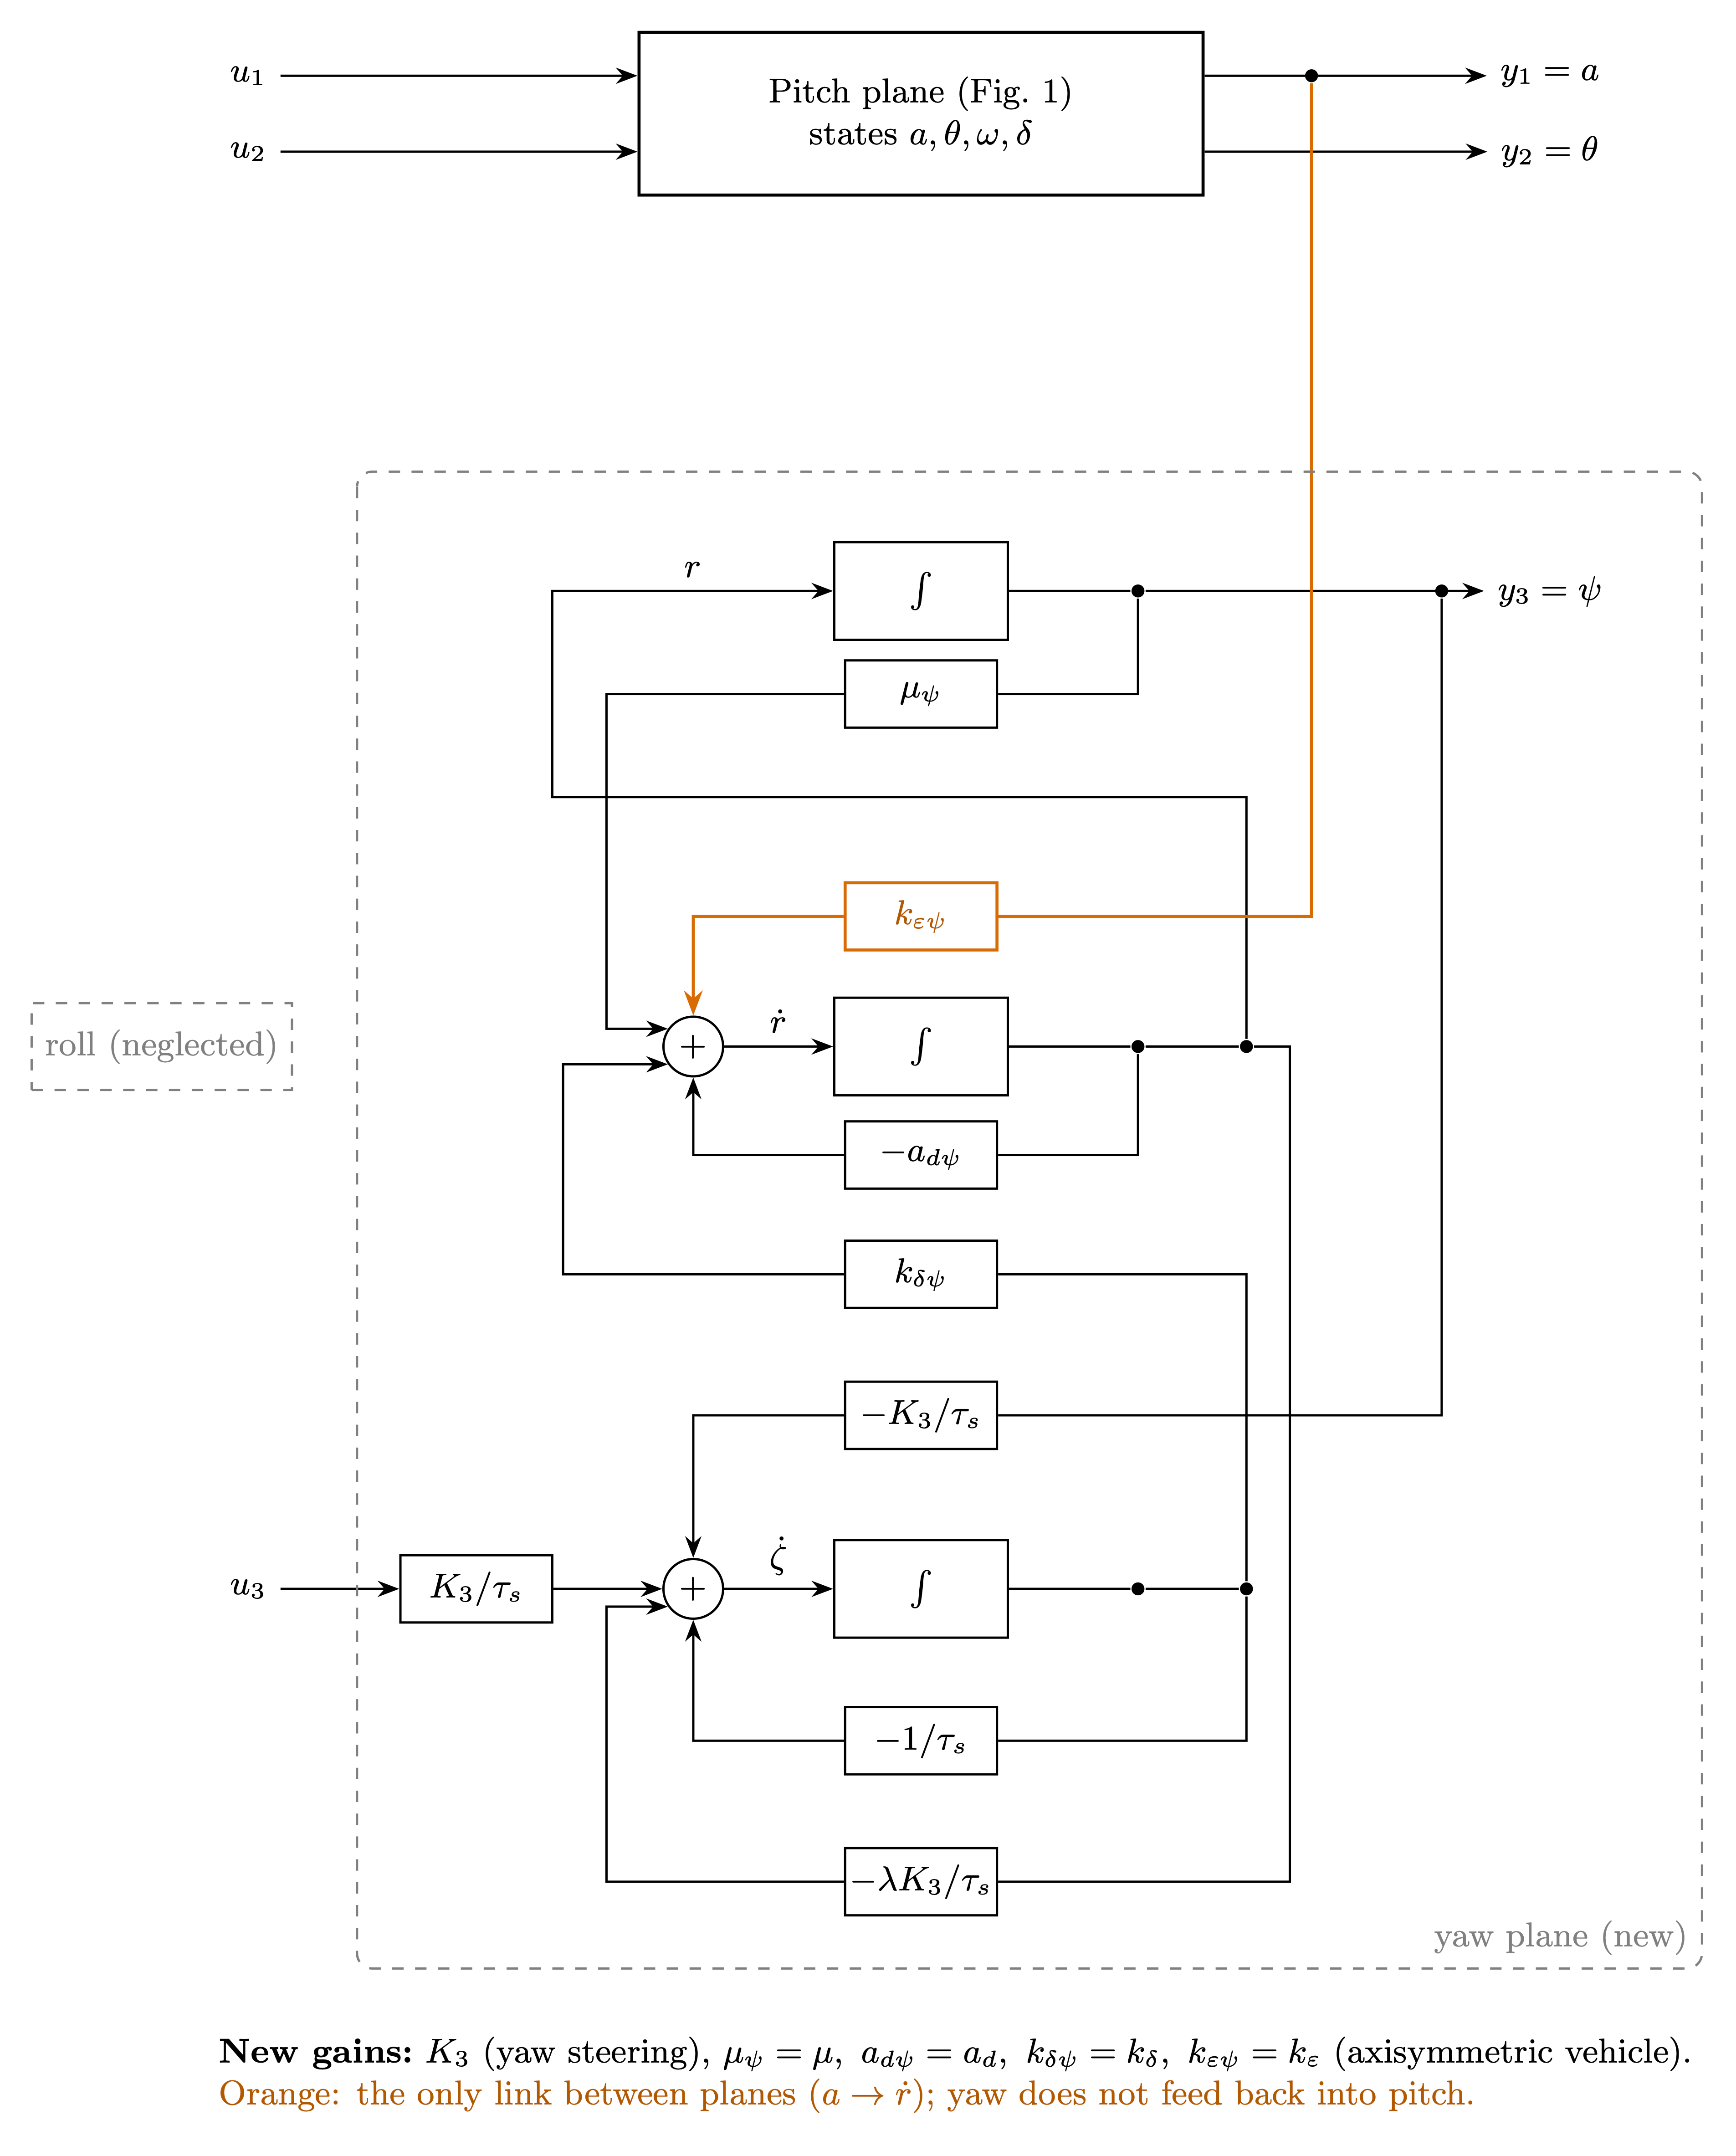
\includegraphics[width=\columnwidth]{fig_f15_yaw.png}
\caption{Diagram with the yaw channel, the pitch plane does not change and the only link between planes is $a\to\dot r$.}\label{fig:yaw}
\end{figure}

Since $A$ is block triangular, its eigenvalues are those of the pitch plane (the ones obtained for the pitch plane) plus three new ones from yaw, so stability is studied separately, the transfer matrix is $3\times3$ with structural zeros, $G_{13}=G_{23}=0$ ($u_3$ moves neither $a$ nor $\theta$) but $G_{31}\ne0$ and $G_{32}\ne0$, since the axial acceleration, which both $u_1$ and $u_2$ move (the latter through gravity), pushes yaw through $k_{\varepsilon\psi}$, the coupling is therefore one-directional, pitch and thrust disturb yaw, but not the other way around, raising $K_1$ increases the coupling $u_1\to\psi$, like $u_1\to\theta$ in pitch, this goes from two to three channels, but it is not yet a complete three-dimensional model, roll is missing, which in a real rocket couples pitch and yaw in both directions, and there is no lateral position either, only orientation.


%====================================================================
\section{Synthesis and Limitations}
\textbf{Instability is the starting point and the nozzle solves it.} Because $\mu>0$ the air tends to overturn the rocket, and only the servo, governed by $K_2$, prevents it, without $K_2$ there is a pole at $+0.557$ s$^{-1}$ and with the servo jammed even the controllability of $\delta$ is lost, $K_2\gtrsim0.09$ is enough to stabilize, and the stability map barely depends on $K_1$, which belongs to a channel that was already stable, this confirms the first part of the hypothesis.

\textbf{Two independent systems or a single MIMO system.} Gravity dominates the coupling, tilting the rocket takes away more acceleration (177\%) than the thrust gives it, while the inverse effect, through the misalignment, is much smaller (21\%), treating the rocket as two independent systems is only reasonable for fast maneuvers, above about 5 rad/s, where both couplings fall below 10\%, for commands that vary slowly the effect of the tilt on the acceleration would be underestimated, the same coupling that gets in the way is what allows the unmeasured states to be \emph{seen}, without it, the rocket would be opaque to the sensors.

\textbf{The effect of $K_1$ and $K_2$.} Each gain has its own job, $K_2$ governs the attitude (damping, rotation speed) and stability, but a high value wastes nozzle and lowers the allowed sampling period, $K_1$ governs how much acceleration is obtained with a thrust command and reduces the gravitational coupling, but increases the inverse coupling, hence a feasible zone and a recommended zone exist bounded by the nozzle (ceiling of $K_2$), by the final error and by the coupling, the result is a compromise.

\textbf{The effect of sampling.} The bandwidth of the rocket ($\sim2$ rad/s) is far below the sampling frequency, so $T=0.05$ s is sufficient with the recommended gains, the limitation is the computation delay combined with high $K_2$, and it gets worse if the mass decreases during flight, which justifies scheduling the gains.

\textbf{Limits of the model.} Everything was obtained with a linear small-angle model, constant parameters, rigid fuselage and steps chosen by the team, the gain recommendation holds for those steps and for the adopted nozzle limit, and with other magnitudes the recommended point shifts, saturations of the engine and of the nozzle, structural flexibility, propellant sloshing and roll were not modeled.

%====================================================================
\section{Conclusion}
A linear MIMO model of the rocket in the pitch plane was studied, the rocket is unstable by nature and the nozzle stabilizes it with $K_2\gtrsim0.09$, with the starting gains $(1,\,0.5)$ the rocket is stable but the gravity coupling is severe (177\%) and the response is slow and oscillatory, the recommended range, $K_1\in[4,\,6.5]$ and $K_2\in[1.1,\,1.45]$, with point $(4.5,\,1.3)$, gives an overshoot of 0.8\%, a settling time of 1.6 s and couplings of 31\% and 28\%, at the cost of using almost the whole nozzle, with two sensors the unmeasured states can be reconstructed, although measuring only $\theta$ is fragile, without the nozzle there is no possible control, a sampling period of 0.05 s is sufficient, the maximum stable period (0.114 s) is 2.3 times larger, even with computation delay, with variable mass the gains should be scheduled with $1/\rho$, and yaw is added as a second plane coupled in a single direction, we learned that the behavior of a multivariable system is better understood by following the physical cause--effect chain than by looking at each channel separately.

%====================================================================
\begin{thebibliography}{9}

\bibitem{nasa}
NASA Glenn Research Center, \emph{Rocket Control. Beginner's Guide to Aeronautics}, \url{https://www1.grc.nasa.gov/beginners-guide-to-aeronautics/rocket-control/}.

\bibitem{nise}
N.~S. Nise, \emph{Control Systems Engineering}, 7th ed., John Wiley \& Sons, 2019.

\bibitem{ogata}
K.~Ogata, \emph{Modern Control Engineering}, 5th ed., Prentice Hall, 2010.

\bibitem{franklin}
G.~F. Franklin, J.~D. Powell and M.~Workman, \emph{Digital Control of Dynamic Systems}, 3rd ed., Addison-Wesley, 1998.

\bibitem{skogestad}
S.~Skogestad and I.~Postlethwaite, \emph{Multivariable Feedback Control: Analysis and Design}, 2nd ed., John Wiley \& Sons, 2005.

\bibitem{wie}
B.~Wie, \emph{Space Vehicle Dynamics and Control}, 2nd ed., AIAA Education Series, 2008.

\bibitem{greensite}
A.~L. Greensite, \emph{Analysis and Design of Space Vehicle Flight Control Systems}, Spartan Books, 1970.

\end{thebibliography}

\end{document}
